\chapter{Literature Review}\label{c:literature}

This chapter reviews recent advancements and current challenges in two key areas relevant to this work: AI-assisted materials discovery (Section \ref{section:section2-1}) and the design of 2D perovskites (Section \ref{section:section2-2}). Particular emphasis is placed on inverse design methodologies within AI-driven approaches and their applicability to the discovery and optimization of 2D perovskite materials. Section \ref{section:section2-3} concludes the chapter by summarizing the literature and identifying key research gaps that motivate the development of the inverse design framework presented in this thesis.

\section{Introduction to AI in Materials Science}\label{section:section2-1}

As introduced in Chapter \ref{c:introduction}, AI has become a transformative tool in materials discovery, often referred to as the “fourth paradigm” of science—complementing experimental, theoretical, and computational approaches (Figure \ref{fig:figure2.1}). This section provides an overview of various AI and machine learning (ML) techniques applied in materials science, with a particular focus on their role in accelerating the discovery of novel materials.


\begin{figure}[ht]
    \centering
    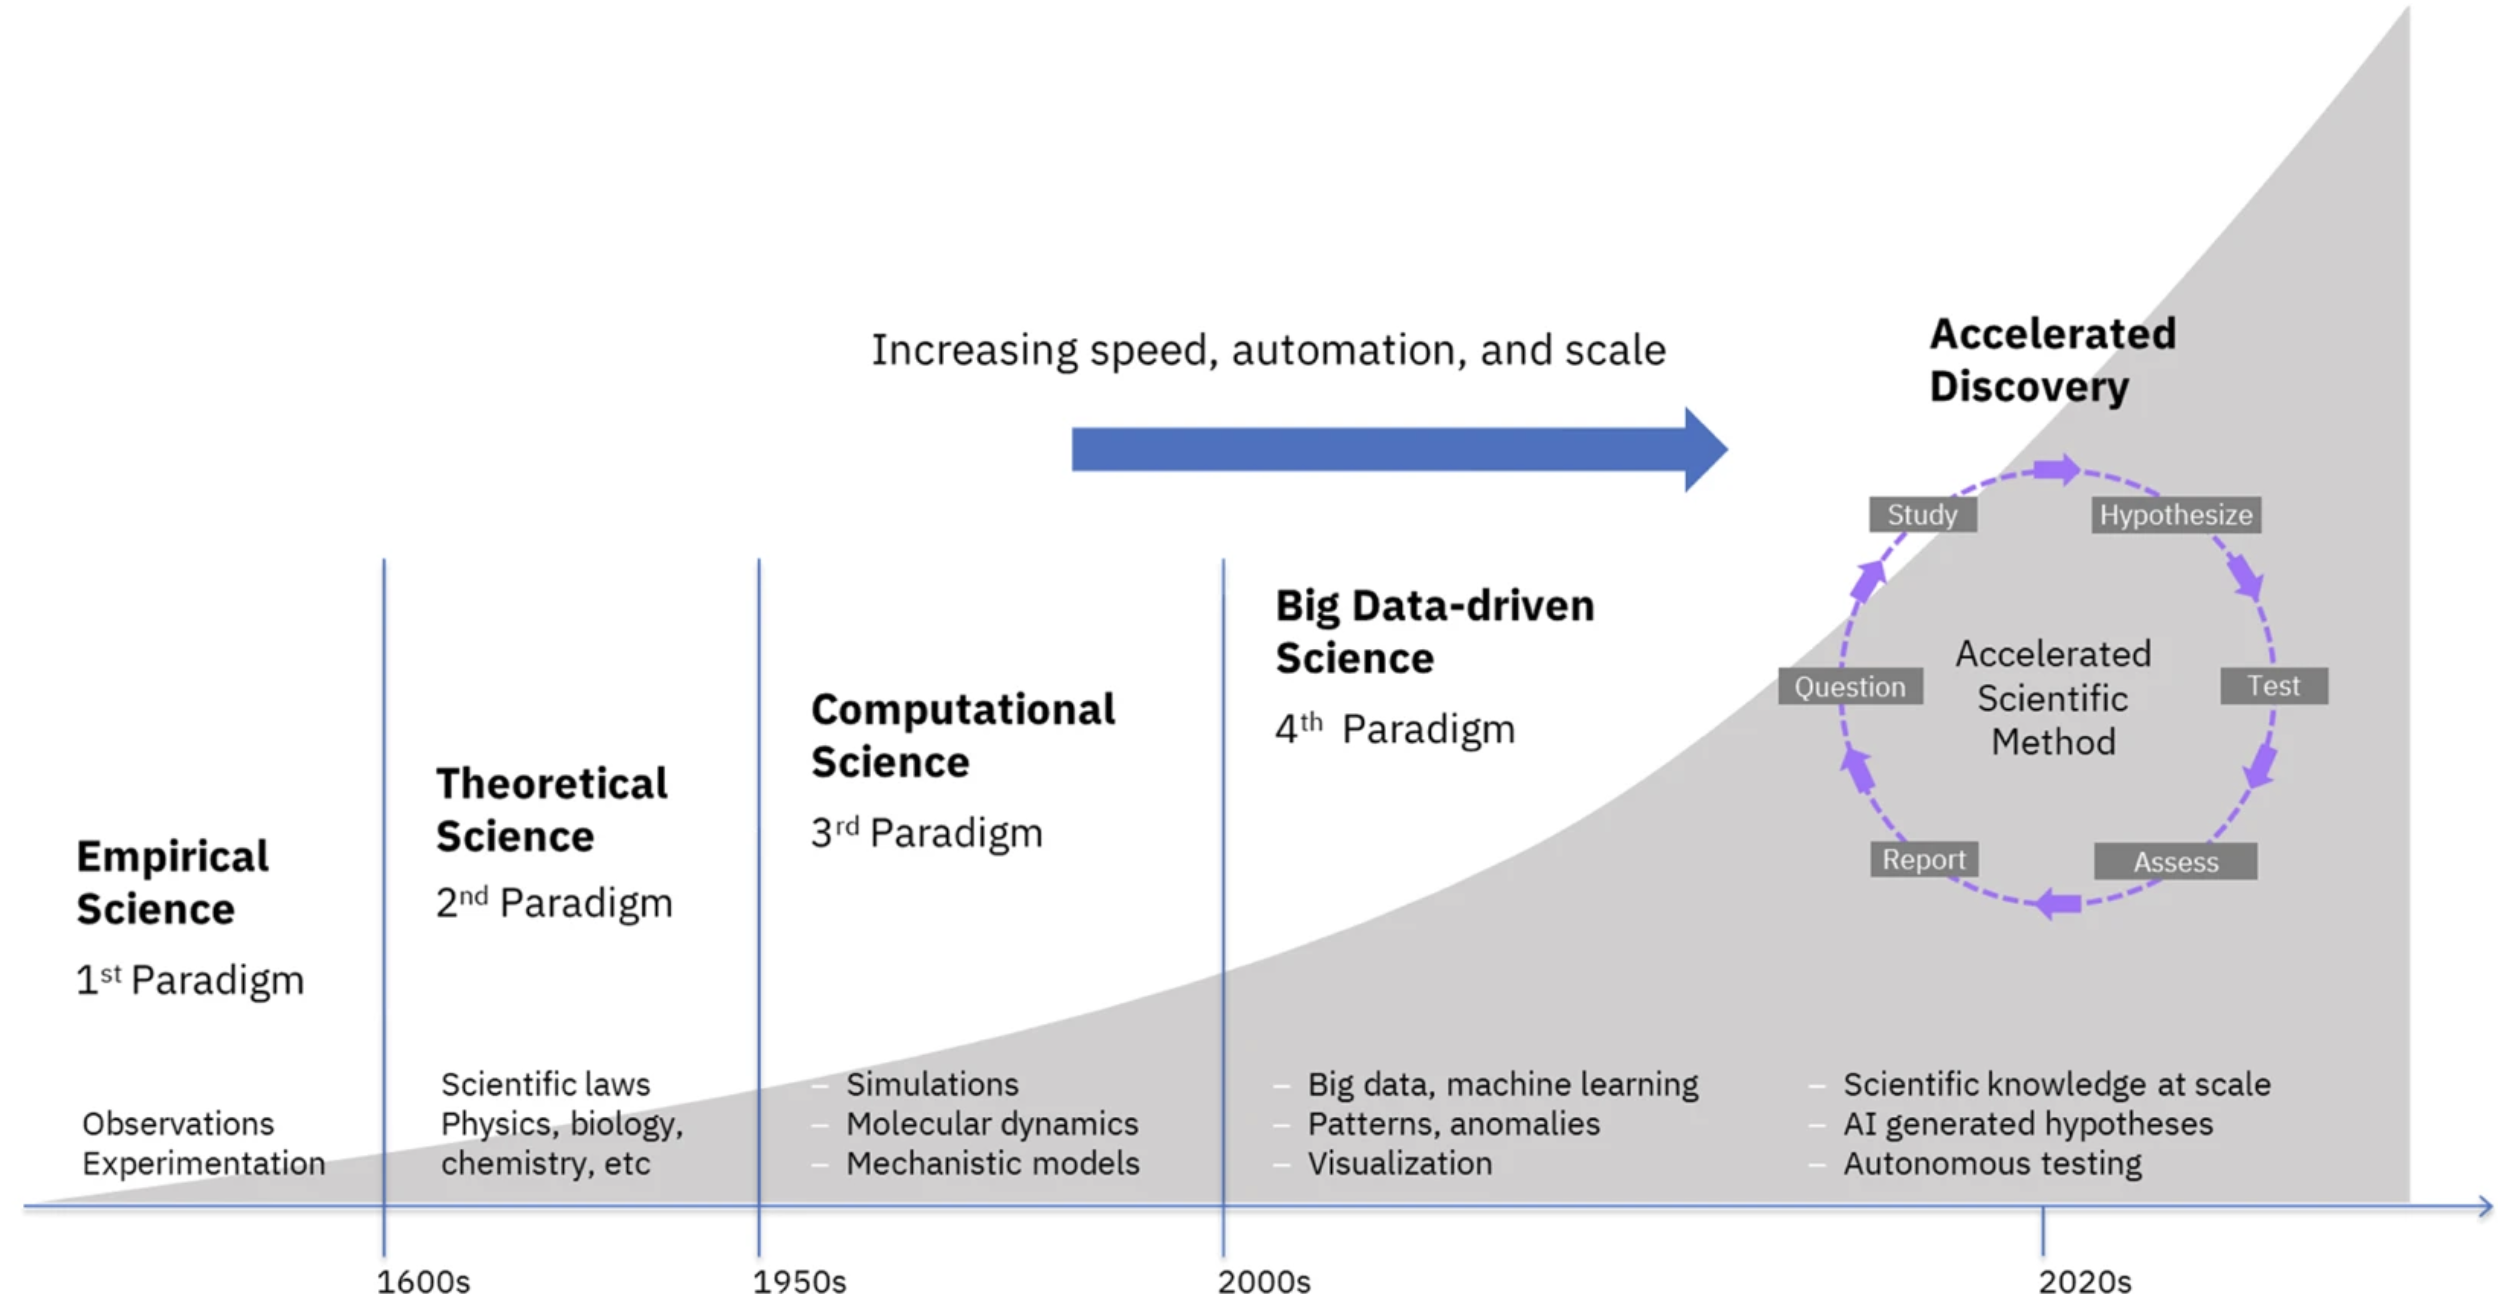
\includegraphics[width=\textwidth]{figures/literature-review/figure2-1.png}
    \caption{The four paradigms of scientific discovery\cite{RN448}.}
    \label{fig:figure2.1}
\end{figure}

The applications of AI in materials science are diverse and rapidly expanding. AI serves as an overarching framework encompassing various concepts, with machine learning (ML) as a key subset specifically applied to materials science. At its core, ML is utilized to identify complex relationships that are either too intricate or computationally expensive for traditional analytical methods\cite{RN318}. Key applications include: 

\begin{enumerate}
  \item Learning structure-property relationships: ML models can predict material properties directly from structural information\cite{RN580,RN556,RN533}. For example, deep learning models have been employed to learn the relationship between the structure of organic molecules encoded in fingerprints and their emission characteristics in light-emitting diodes\cite{RN66}. For inorganic materials, deep learning model has been used to model the relationship between the composition of high-entropy alloys and their thermal expansion coefficients\cite{RN532}. 
  
  \item Optimizing synthesis parameters: AI can elucidate reaction mechanisms and optimize experimental conditions for complex chemical reactions\cite{,RN341,RN574,RN552,RN581}. Supervised ML models have been trained to correlate synthesis parameters with reaction outcomes, enabling the efficient design of experiments and reducing the trial-and-error typically associated with materials synthesis\cite{RN328}. 
  
  \item Accelerating computational methods: AI models can reduce the computational cost of traditional simulation techniques. For instance, active learning models have been developed to perform quantum mechanical calculations using small to medium-sized molecular building blocks instead of individual atoms, as in first-principles methods. These models have demonstrated faster and reliable predictions across diverse material systems and target properties\cite{RN561}.
  
\end{enumerate}

Given the broad range of AI applications in materials science, this literature review chapter focuses specifically on machine learning for materials discovery. This domain often encompasses one or more of the scenarios discussed above, with the primary goal of identifying novel or previously unexplored materials that exhibit superior properties compared to existing ones. In the following sections, we provide a systematic framework to clarify the various ML methods employed in materials discovery, addressing the diverse terminologies commonly found in the literature. Additionally, we will discuss how these ML methods can be integrated into a comprehensive machine learning workflow and how they can be effectively combined with other data-driven approaches to enhance materials research.




\subsection{Types of ML methods used for materials discovery}

\begin{figure}[ht]
    \centering
    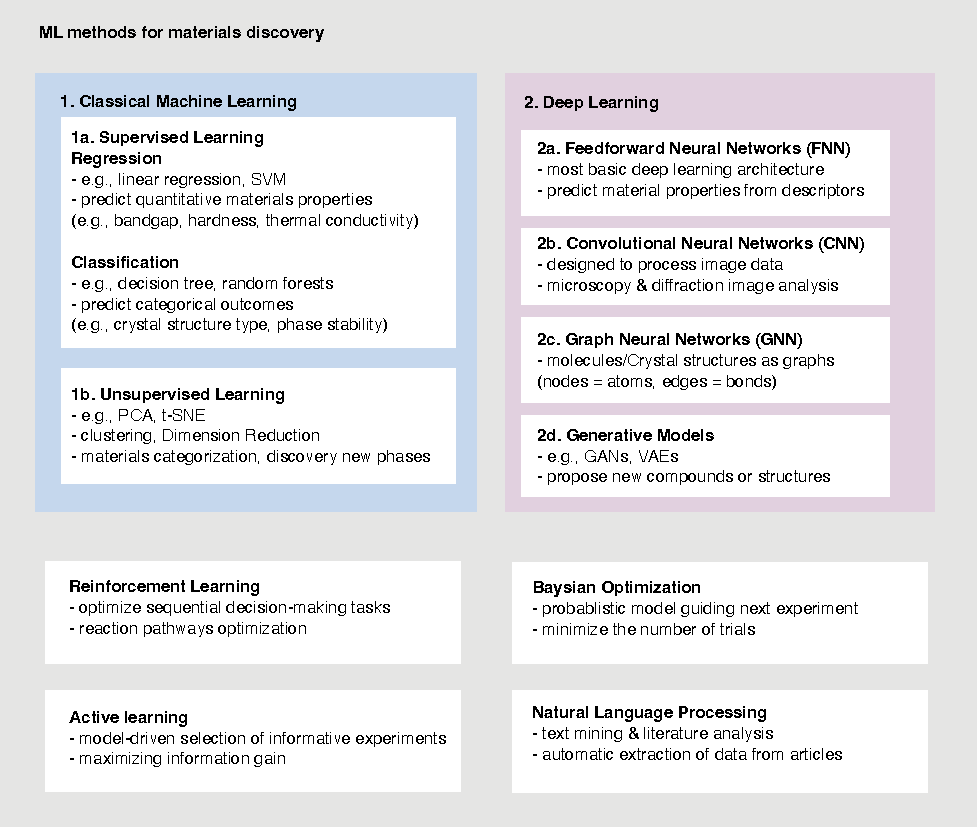
\includegraphics[width=\textwidth]{figures/literature-review/figure2-2.pdf}
    \caption{Common types of ML methods typically used in materials science.}
    \label{fig:figure2.2}
\end{figure}

An overview of commonly used ML methods is summarized in Figure \ref{fig:figure2.2}. Within ML, approaches that rely on manually engineered features and relatively simple model architectures are referred to as classical ML methods, with supervised learning being one of the earliest and mostly widely used techniques. The first notable application of supervised learning in materials science dates back to 2010, where a probabilistic model is built to identify the most probable crystal structures of unseen ternary oxide compounds\cite{RN542}. Classical ML methods remain widely used, particularly when dealing with smaller datasets (typically below thousands of data points) or when model interpretability is a key priority. Meanwhile, deep learning represents a specialized branch of ML that employs multi-layered neural networks capable of automatically extracting features from raw data. Unlike classical ML methods, deep learning does not require manual feature engineering, as it can learn hierarchical representations directly from input data. Deep learning methods have become increasingly popular in materials science due to their superior performance in tasks involving large and high-dimensional datasets. However, DL methods typically require larger datasets (often exceeding $\sim10,000$ data points), significant computational resources, and can be less interpretable compared to classical ML approaches.

\textbf{Classical Machine Learning}

The most distinctive types of classical ML methods are supervised and unsupervised learning.
In supervised learning, models are trained on labelled datasets, where each data point is associated with a known outcome, such as a material property (for regression tasks) or a class label (for classification tasks). 
\begin{itemize}
    \item Regression models, such as linear regression, random forests, Gaussian process regression, and support vector regression (SVR), are used to map input descriptors (e.g., elemental fractions, lattice parameters) to quantitative material properties such as bandgap, thermodynamic stability, and morphology\cite{RN563,RN593,RN317,RN13}. For instance, a random forest regression model has been employed to correlate the elemental composition of adsorption sites with the electrocatalytic adsorption energy of copper-containing intermetallic crystals\cite{RN551}. 

    \item Classification techniques such as logistic regression, support vector machines (SVMs), decision trees are designed to predict discrete labels. These models are commonly applied to tasks such as phase classification, crystal structure identification, and synthesizability prediction\cite{RN315,RN580,RN321}. For example, various classification models have been used to distinguish between different oxidation states in metal-organic frameworks (MOFs) based on local environmental features, including metal type, coordination geometry, and chemical environment\cite{RN580}.
    
\end{itemize}

Supervised learning approaches excel when reliable labelled data is available, whether from experimental measurements or computational simulations. They are typically more interpretable and computationally efficient compared to many deep learning models, making them attractive for iterative property prediction and materials design workflows.

In unsupervised learning, the objective is to uncover hidden patterns or groupings within unlabelled data without predefined outcomes. 

\begin{itemize}
    \item Clustering algorithms like k-means clustering, hierarchical clustering, and Gaussian mixture models are employed to group materials with similar feature profiles, potentially revealing unexpected trends or novel material families\cite{RN571,RN555}. For example, a study applied hierarchical agglomerative clustering to categorize ternary nitrides into distinct chemical families based on their stability and metastability profiles\cite{RN555}.
    \item Dimensionality reduction techniques, including principal component analysis (PCA) and t-distributed stochastic neighbour embedding (t-SNE), are used to project high-dimensional materials data into lower-dimensional spaces. This facilitates the visualization of patterns, identification of outliers, and discovery of structure–property relationships that might be obscured in higher dimensions\cite{RN412,RN574,RN551}.
\end{itemize}

By revealing latent structures in the data, unsupervised methods can provide valuable insights into structure–property correlations and guide targeted experimental or computational investigations.

\textbf{Deep Learning}

Deep learning (DL) is a specialized branch of ML that employs multi-layered neural networks to automatically learn features from raw data. This approach significantly reduces the need for manual feature engineering, provided that sufficient training data and computational resources are available. DL models excel at capturing complex, non-linear relationships in high-dimensional datasets, making them particularly valuable for a wide range of materials science applications.

Feedforward neural networks (FNNs) represent the most basic form of deep learning architecture. In these models, information flows in a single direction—from input to output—through multiple layers of interconnected nodes (neurons). FNNs are effective for both regression and classification tasks, particularly when datasets are large enough to support the direct learning of representations from raw inputs, such as the chemical structures of organic molecules\cite{RN581,RN610}. In one of the earliest applications of deep learning in materials science, a simple neural network architecture with two hidden layers—the minimum number required to be classified as deep learning—was used to design organic molecules for light-emitting diode (LED) applications\cite{RN66}. While more advanced deep learning architectures have since been developed, FNNs are often employed as baseline models for benchmarking the performance of more complex networks.

Convolutional neural networks (CNNs) are designed to process grid-like data structures, such as images, by applying convolutional filters that automatically detect spatial hierarchies and local patterns. In materials science, CNNs are widely used for analysing image-based datasets, including microscopy images (e.g., SEM, TEM) to identify microstructural features or defect distributions and diffraction patterns for automated phase classification and structural analysis\cite{RN550,RN604,RN564}. For example, a CNN architecture with six convolutional layers was developed to classify crystal phases from X-ray diffraction (XRD) patterns automatically\cite{RN604}.

Graph neural networks (GNNs) are particularly well-suited for materials science because they natively process graph-structured data, which naturally represents molecules and crystal structures. In this framework, atoms are represented as nodes, and bonds or interatomic interactions are represented as edges. GNNs have demonstrated remarkable success in predicting a wide range of material properties, including crystal stability, electronic properties, and surface chemistry\cite{RN336,RN562,RN362}. A notable example is GNoMe, a state-of-the-art AI model developed by Google DeepMind, which uses GNNs to predict and discover new crystalline materials. GNoMe has achieved unprecedented scalability, significantly improving the efficiency of materials discovery—reportedly accelerating the process by an order of magnitude\cite{RN601}.

Generative models aim to create new data samples that resemble the distribution of existing data, making them highly effective for inverse materials design. Two widely used generative models in materials science include Generative Adversarial Networks (GANs) and Variational Autoencoders (VAEs). Generative models can propose novel materials with desired properties, such as targeted band gaps, thermal conductivity, or mechanical strength\cite{RN326,RN532,RN412}. For instance, MatterGen, a generative AI model developed by Microsoft Research, represents a significant breakthrough in materials science\cite{RN633}. It enables the design of new inorganic materials with specific target properties, greatly accelerating the exploration of vast compositional spaces.

\textbf{Other Machine Learning Methods}

Active learning is especially valuable when experimental or simulation data are scarce or expensive to obtain. In this method, the model autonomously selects the most informative data points or experiments to label next, thereby optimizing the learning process with minimal resources. Active learning strategies are often integrated with Gaussian process regression (GPR), due to its inherent uncertainty quantification, or neural networks to target high-uncertainty regions in the materials design space. This approach rapidly converges on optimal candidates while minimizing total experimental cost\cite{RN601, RN604, RN551,RN532}.

In contrast to methods that rely on static datasets, reinforcement learning (RL) focuses on sequential decision-making, where an agent explores chemical or process pathways and receives “rewards” for achieving specific outcomes (e.g., synthesizing a stable or high-performing material). RL is particularly powerful in dynamic laboratory environments, enabling autonomous experimentation through real-time tuning of synthesis parameters and adaptive control of reactors. This exploration-exploitation framework allows RL to discover novel materials and optimize processes beyond human intuition\cite{RN604,RN339}.
Bayesian optimization employs probabilistic models to iteratively recommend the next most promising experiments based on current knowledge and uncertainty. By leveraging acquisition functions—such as expected improvement or upper confidence bound—these methods balance exploration and exploitation to efficiently identify parameter sets or compositions with superior properties (e.g., optimized reaction yield or solar cell efficiency)\cite{RN549,RN362,RN612}.

Natural language processing (NLP) facilitates large-scale text mining of scientific literature, patents, and databases to extract valuable information, including synthesis protocols, property data, and structure-property relationships. Recent advances, particularly transformer-based models, have enhanced the ability to capture complex semantic patterns. When combined with knowledge graph construction, NLP can reveal hidden correlations, accelerate hypothesis generation, and guide experimental design toward previously unexplored materials spaces\cite{RN604,RN635,RN634,RN636}.

\subsection{Incorporation into Materials Discovery Workflows}

\begin{figure}[ht]
    \centering
    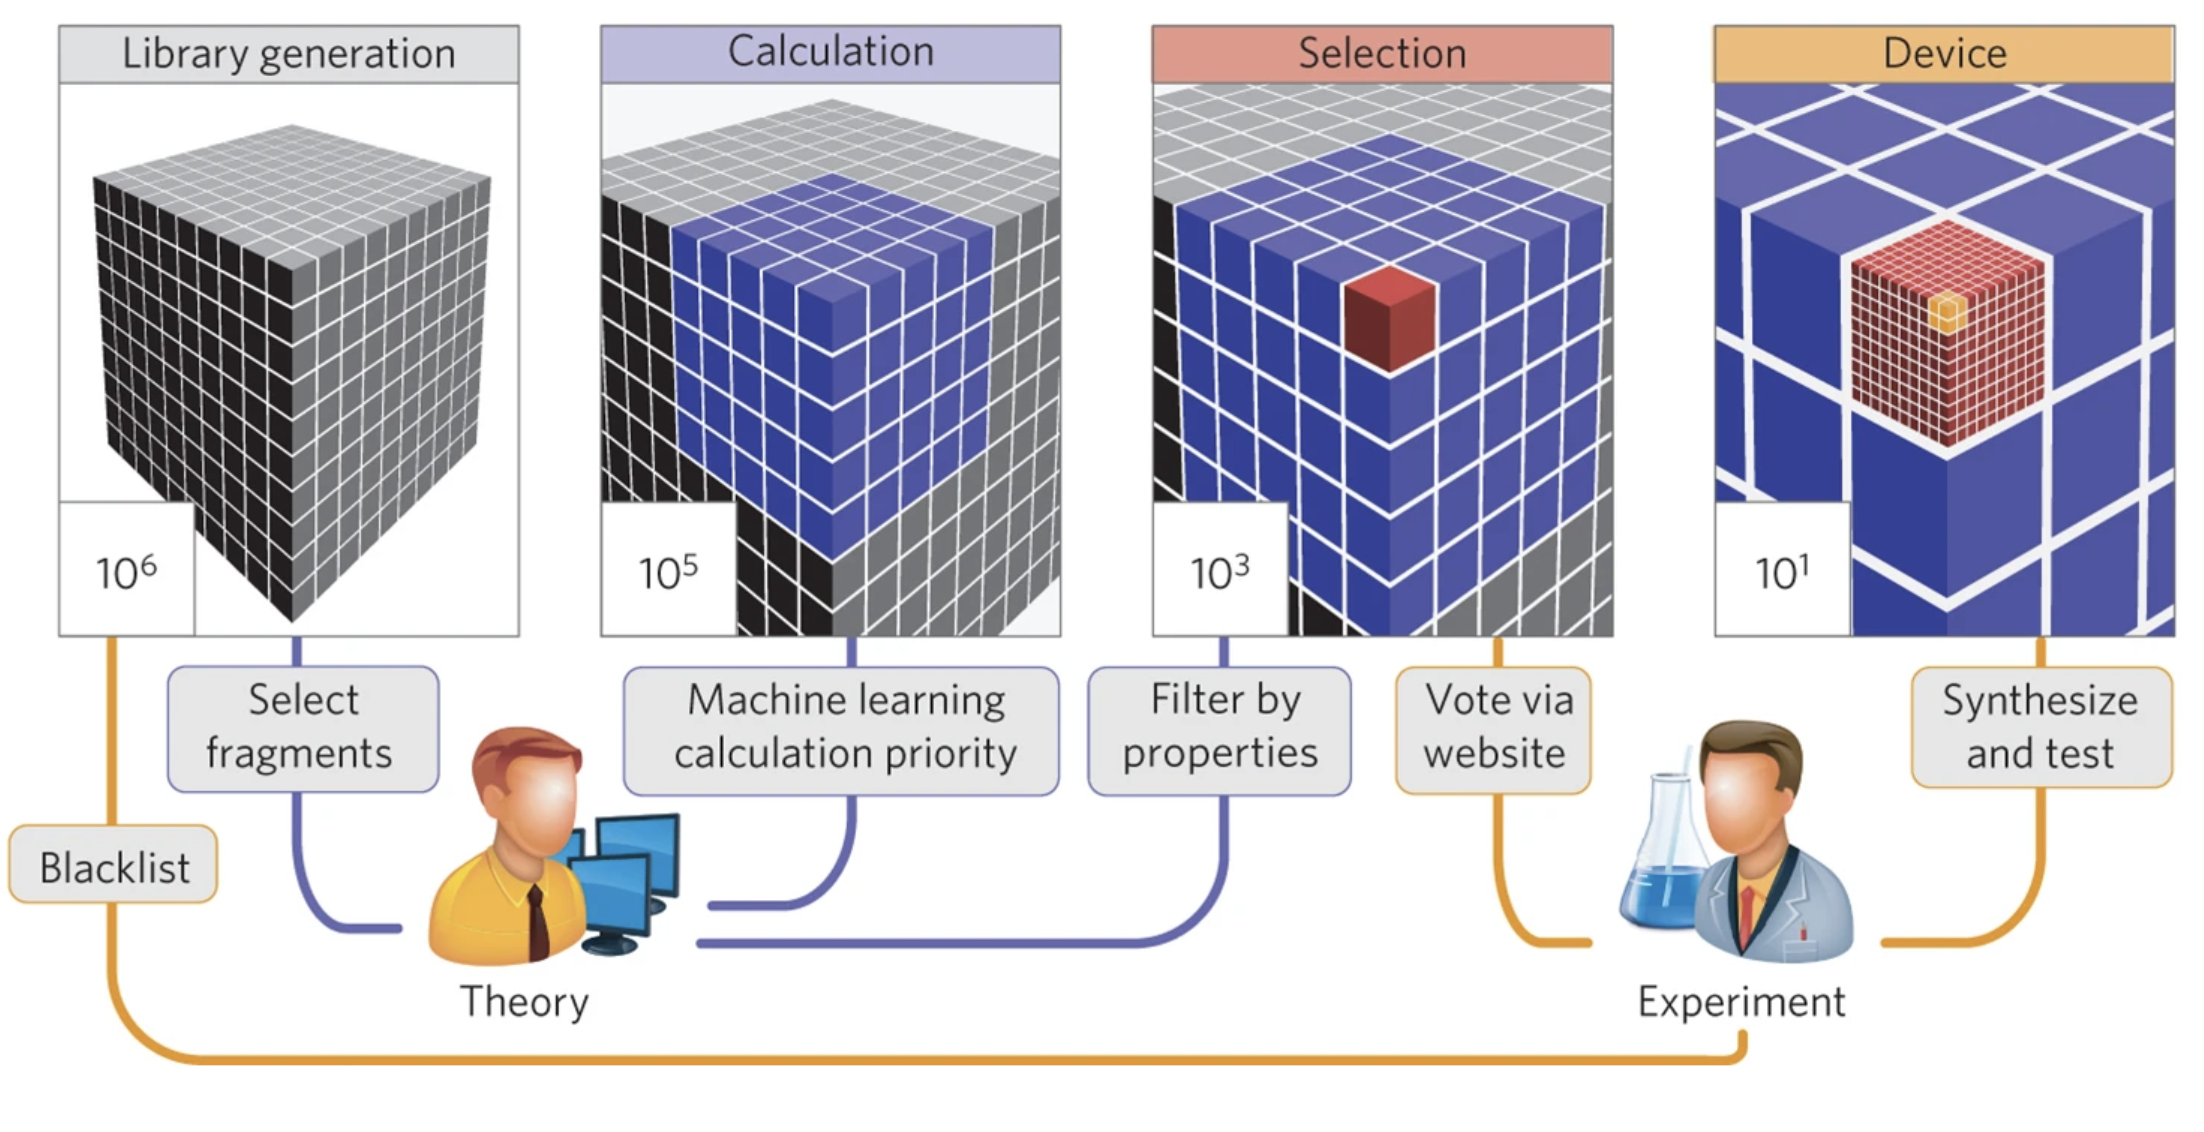
\includegraphics[width=\textwidth]{figures/literature-review/figure2-3.png}
    \caption{A ML-assisted materials discovery workflow in an early OLED study\cite{RN66}.}
    \label{fig:figure2.3}
\end{figure}

Building on the discussion of ML methods used in materials discovery, this section explores how ML is seamlessly integrated into materials discovery pipelines. Since ML models require large datasets to learn effectively, they are often combined with high-throughput computational tools and experimental platforms to generate the necessary training data.

On the computational side, large-scale density functional theory (DFT) and molecular dynamics (MD) simulations serve as key sources of labelled datasets for ML model training and fine-tuning. These simulations help establish structure–property relationships, enabling models to make more accurate predictions. Meanwhile, on the experimental side, automated synthesis and characterization platforms generate high-quality data that can be continuously fed back into ML models. This iterative process forms a closed-loop system where predictions guide experiments, and experimental outcomes, in turn, refine the model, accelerating the materials discovery cycle.

One of the earliest examples of ML integration in materials discovery was demonstrated in a 2016 study on organic light-emitting diode (OLED) materials\cite{RN66}. In this work, a simple deep learning model with just two hidden layers was incorporated into a materials discovery workflow that included materials generation, high-throughput calculations, virtual screening, and experimental fabrication (Figure \ref{fig:figure2.3}). This streamlined workflow identified thousands of promising candidates, and subsequent experimental validation revealed several materials with exceptionally high quantum efficiency, showcasing the predictive power and practical utility of ML-enhanced discovery pipelines.

\begin{figure}[ht]
    \centering
    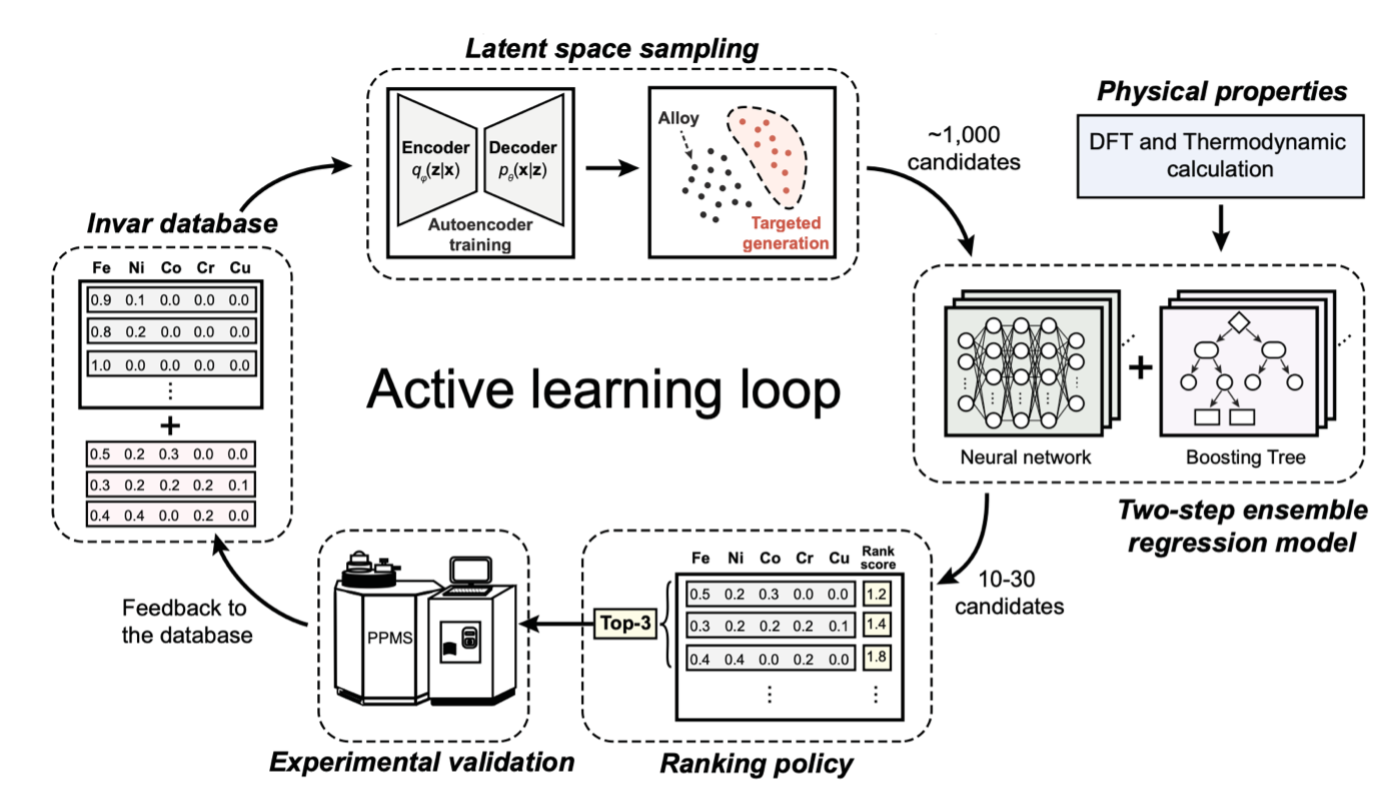
\includegraphics[width=\textwidth]{figures/literature-review/figure2-4.png}
    \caption{An active learning loop applied to high-entropy alloy discovery\cite{RN532}.}
    \label{fig:figure2.4}
\end{figure}

A more advanced example is the discovery of high-entropy alloys (HEAs) as shown in Figure \ref{fig:figure2.4}, where an active learning framework was developed, integrating ML with high-throughput DFT calculations, thermodynamic modelling, and experimental synthesis\cite{RN532}. At the core of this workflow, a generative model proposed new compositions, while a custom two-step regression model predicted their properties. Out of millions of potential compositions, 17 new alloys were synthesized and characterized, leading to the identification of two HEAs with targeted thermal expansion properties.


\begin{figure}[ht]
    \centering
    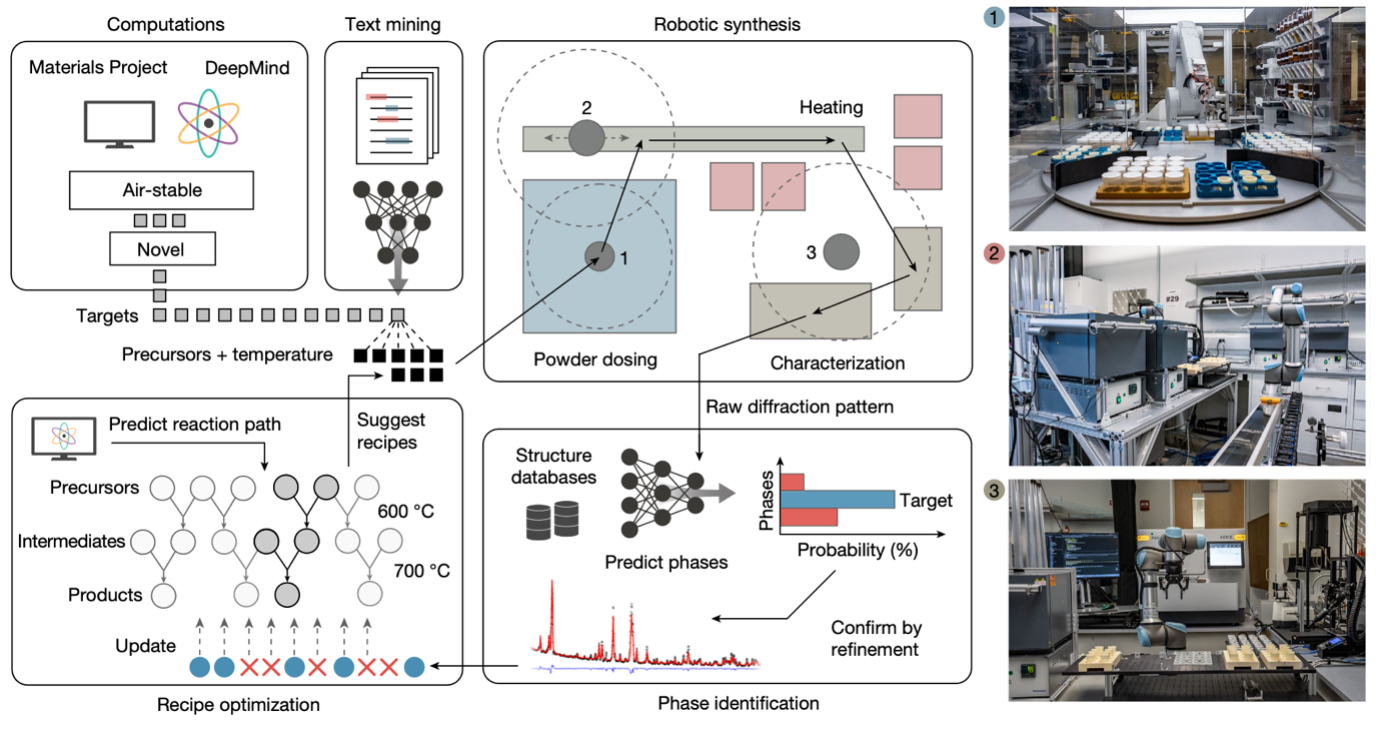
\includegraphics[width=\textwidth]{figures/literature-review/figure2-5.png}
    \caption{Automated materials discovery with the A-Lab platform\cite{RN604}.}
    \label{fig:figure2.5}
\end{figure}

At the highest level of complexity, fully autonomous materials discovery systems are emerging, integrating multiple AI models into unified closed-loop frameworks. A notable example is the A-Lab platform (Figure \ref{fig:figure2.5}), which employs several ML models to accelerate discovery\cite{RN604}. First, an NLP model is trained on extensive databases of synthesis procedures extracted from the literature. This is followed by a regression model that predicts optimal synthesis temperatures based on precursor materials. When initial synthesis attempts are unsuccessful, an active learning algorithm iteratively refines the synthesis parameters using experimental feedback. Finally, convolutional neural networks (CNNs) are employed to analyse X-ray diffraction (XRD) patterns of the synthesized materials, aiding in the rapid identification of successful synthesis outcomes.

\subsection{Inverse Design in Materials Discovery}

\begin{figure}[ht]
    \centering
    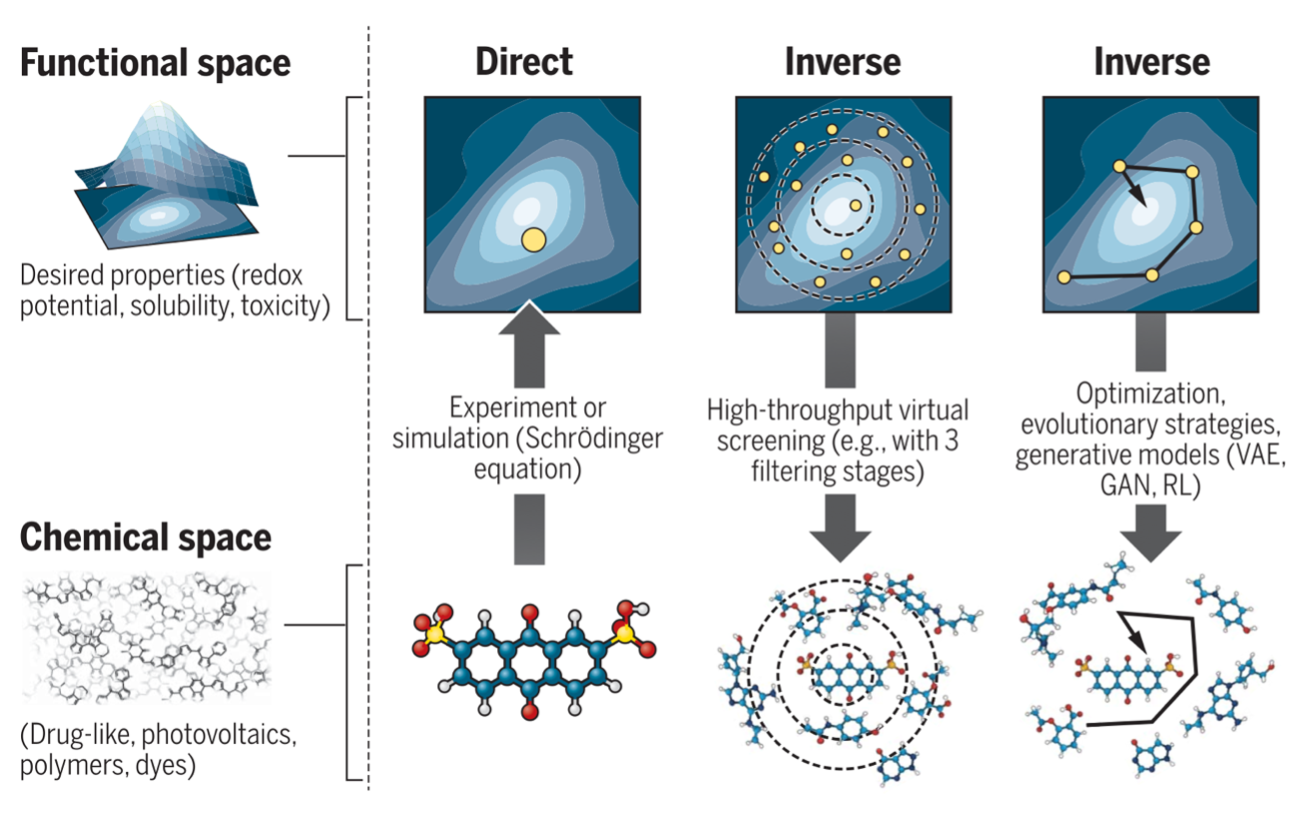
\includegraphics[width=\textwidth]{figures/literature-review/figure2-6.png}
    \caption{Overview of direct and inverse approaches in materials discovery\cite{RN361}.}
    \label{fig:figure2.6}
\end{figure}

Building upon the integration of ML into materials discovery workflows, an even more ambitious application is inverse design, often regarded as a significant milestone—or even the “holy grail”—of materials discovery. Rather than adopting the traditional forward or direct-design approach of starting with a known material and then determining its properties, inverse design begins by specifying target properties or functionalities (Figure \ref{fig:figure2.6}). Computational methods are then used to identify, generate, or suggest materials that fulfill these specifications. This property-oriented framework is poised to efficiently traverse the vast chemical and structural space, thereby minimizing trial-and-error experimentation and accelerating the discovery of novel materials with precise functionalities\cite{RN361,RN547}.

Although the concept of inverse design has been discussed for several decades, the rapid rise of ML in materials science has significantly advanced its practical implementation. Thanks to ML’s capacity to model high-dimensional data and capture complex structure–property relationships, inverse design workflows have become more robust and predictive, offering the potential for real-world applicability in diverse materials domains.

Despite its growing popularity, inverse design does not yet have a universally agreed-upon definition within the materials science community. Some methodologies that effectively implement an inverse design workflow do not explicitly label themselves as such. For instance, while high-throughput screening (HTS) is often considered part of forward discovery, some researchers classify it as a subset of inverse design. These terminological distinctions highlight the evolving nature of the field, but the fundamental principle of inverse design remains unchanged: instead of starting with a known material and analysing its properties, we begin with a desired property and work backward to identify suitable structures or compositions. 

Three primary methodologies are commonly used in inverse design: (1) generative models, (2) iterative design strategies (e.g., active learning, Bayesian optimization, genetic algorithms), and (3) invertible materials representations. Among these, generative models and invertible representations take a fundamentally different approach from iterative techniques. While iterative methods refine candidate materials through sequential optimization loops, generative models and invertible representations aim to construct viable materials from scratch based on predefined target properties. By leveraging these approaches, researchers can efficiently explore vast chemical spaces and propose entirely new material candidates, rather than incrementally improving known ones. This ability to generate novel structures directly from property requirements makes these methods particularly valuable for inverse design. The following sections provide an in-depth overview of generative models and invertible materials representations, examining their respective strengths, limitations, and distinct roles in accelerating materials discovery.

\begin{figure}[ht]
    \centering
    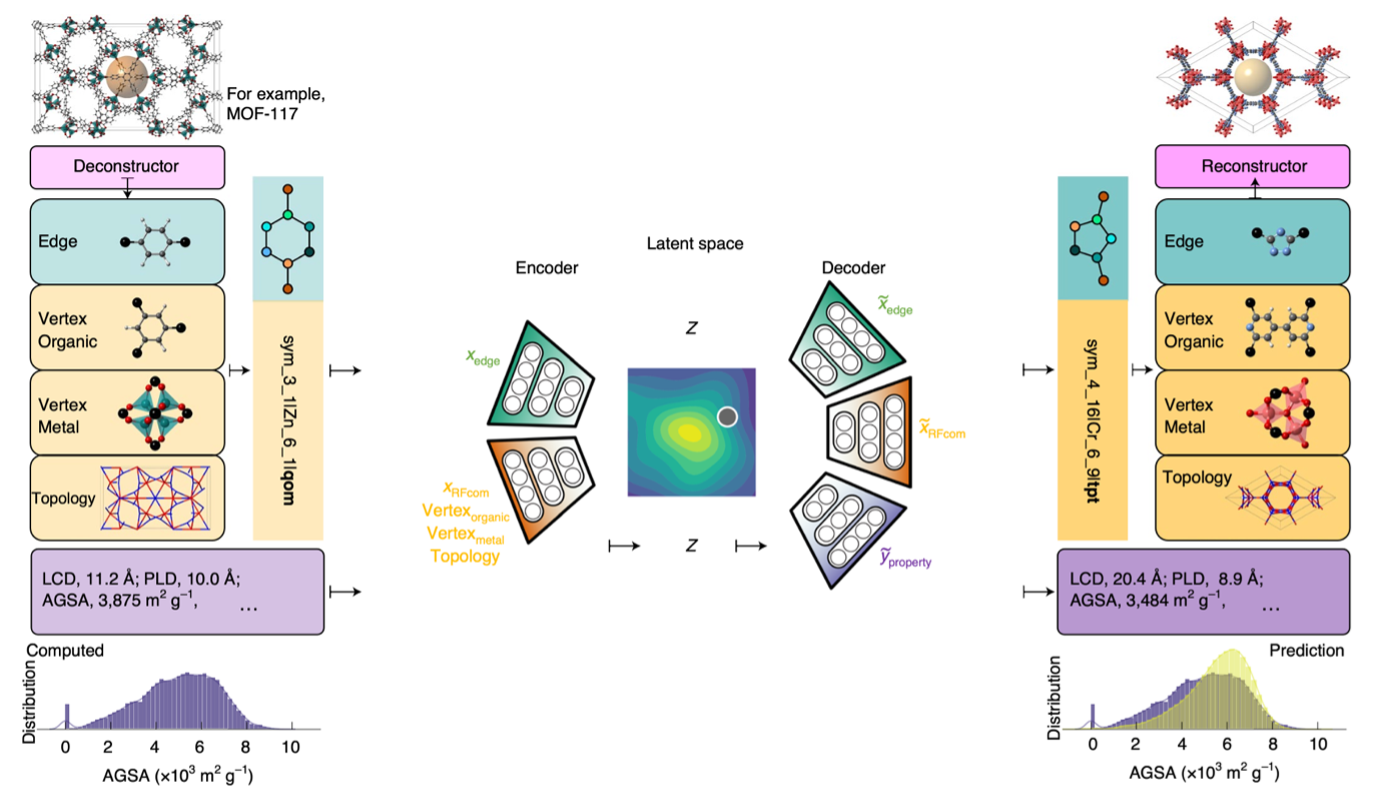
\includegraphics[width=\textwidth]{figures/literature-review/figure2-7.png}
    \caption{Schematic representation of a typical generative model workflow\cite{RN412}.}
    \label{fig:figure2.7}
\end{figure}

\textbf{Generative models}

Generative models including Variational Autoencoders (VAEs) and Generative Adversarial Networks (GANs), have emerged as powerful techniques for inverse design\cite{RN412, RN633, RN347, RN614, RN70}. In these frameworks, models learn probabilistic distributions over existing materials or molecules. Once trained, they can generate new candidate structures or compositions that are likely to exhibit desired properties, effectively “mapping” targeted characteristics back to plausible chemical formulas or structural motifs. These methods are particularly impactful in organic molecule design (e.g., pharmaceuticals, organic semiconductors), where a dense, high-quality dataset of known molecules can be leveraged to yield innovative new candidates. 

One of the earliest notable demonstrations of a generative model in materials discovery was a VAE architecture composed of an encoder and decoder using recurrent neural networks, designed to generate organic molecules\cite{RN411}. Since then, generative models have been applied across various material classes. For example, they have been used to generate novel metal–organic frameworks (MOFs) with exceptional gas separation properties\cite{RN412}. More recently, MatterGen, a generative model introduced by Microsoft, has demonstrated the ability to generate stable and diverse inorganic materials spanning the entire periodic table. Moreover, it can be fine-tuned to design materials with specific target properties\cite{RN633}. 

Despite these successes, the application of generative models remains largely limited to material classes with relatively well-defined structures and abundant training data. Their implementation in highly constrained materials systems, such as the organic spacers in 2D perovskites, is still rare. This limitation may stem from the scarcity of high-quality datasets in these domains, which restricts the model’s ability to learn meaningful structure–property relationships. Without sufficient domain knowledge or physics-based constraints integrated into the learning process, generative models struggle to propose viable candidates in these more complex materials spaces. Addressing these challenges will be crucial for expanding the scope of inverse design methodologies to a broader range of materials.

\textbf{Invertible Material Representations}

A growing area of research focuses on developing bidirectional mappings between material representations and desired property spaces\cite{RN354,RN599}. Unlike many black-box models that learn an inverse mapping implicitly, invertible representations provide a more transparent and structured approach to inverse design. This enables researchers to start in the property domain and systematically work backward to identify candidate structures, making the design process more interpretable and controllable. For molecular systems, several well-established invertible representations exist, including simplified molecular-input line-entry system (SMILES), international Chemical Identifier (INCHI) and molecular graph\cite{RN648}. These representations allow machine learning models to efficiently encode molecular structures and generate new candidates based on specified properties. 

\begin{figure}[ht]
    \centering
    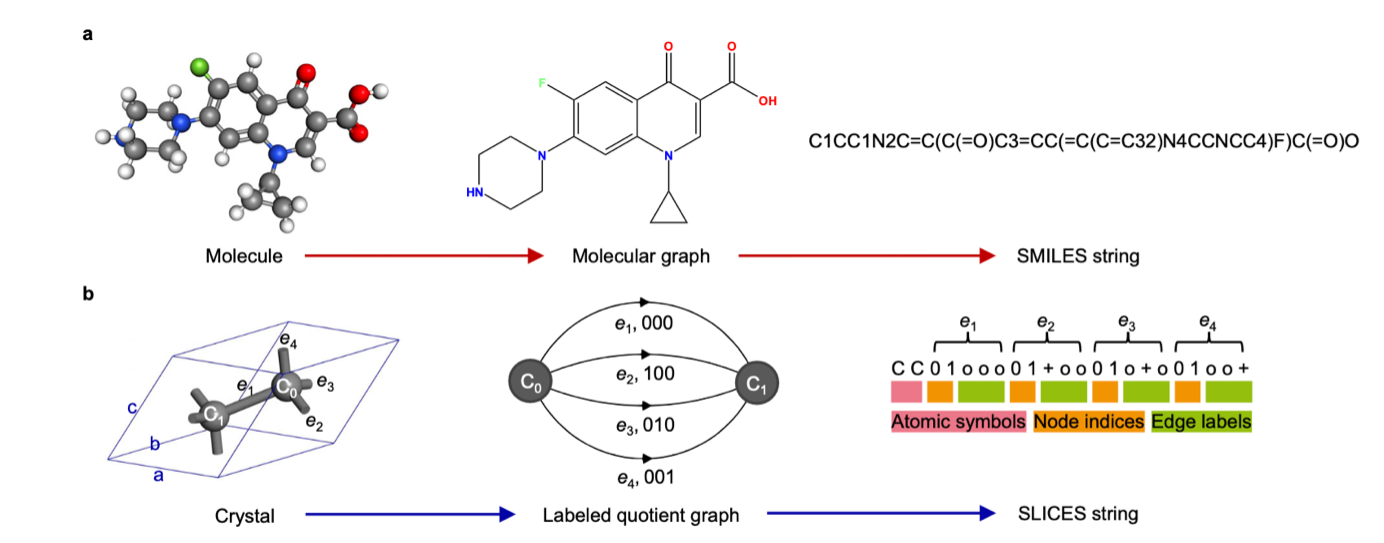
\includegraphics[width=\textwidth]{figures/literature-review/figure2-8.png}
    \caption{Invertible representations in molecular systems and solid-state crystals\cite{RN642}.}
    \label{fig:figure2.8}
\end{figure}

For inorganic crystals, the development of invertible representations is more challenging. Unlike molecules, where connectivity can be described in a straightforward manner, solid-state materials require a representation that captures both periodicity and compositional complexity. This has been a longstanding challenge in materials informatics, as achieving invertibility while maintaining generalizability and property-driven design remains difficult. Several representations have been proposed to address this issue, but none have yet become universal standard\cite{RN642,RN354}.

Despite these challenges, invertible material representations have significant potential in inverse design, particularly when used in conjunction with machine learning models. By establishing structured and reversible mappings between materials and their properties, these representations provide a powerful framework for rational material generation, facilitating more efficient and targeted discovery.

\section{2D Hybrid Perovskites}\label{section:section2-2}

Two-dimensional (2D) hybrid perovskites have emerged as a fascinating class of materials that combine the desirable optoelectronic properties of their three-dimensional counterparts with enhanced chemical and environmental stability. In general, these materials consist of inorganic metal halide layers separated by organic cations, creating a naturally layered architecture. By tuning the thickness of these inorganic layers or altering the organic interlayers, researchers can tailor properties such as bandgap, exciton binding energy, and overall structural stability. Thus, 2D perovskites have attracted attention for applications ranging from solar cells and light-emitting diodes to photodetectors and field-effect transistors\cite{RN108}.

Unlike 3D perovskites, where small organic cations (e.g., methylammonium or formamidinium) fit within the perovskite lattice, 2D perovskites incorporate larger organic spacer molecules that enforce a layered structure and introduce new functionalities. This dimensional reduction results in strong quantum confinement effects, leading to distinct optical and electronic behaviours compared to their 3D analogy. In the following subsections, we discuss the structural variations of 2D perovskites, focusing on key phase families, and explore their fundamental electronic properties.

\subsection{Structural and Electronic Fundamentals}

\begin{figure}[ht]
    \centering
    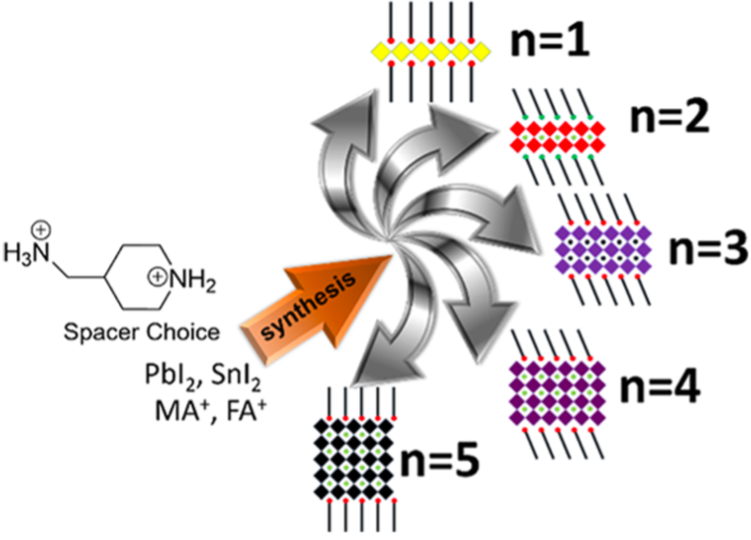
\includegraphics[width=0.6\textwidth]{figures/literature-review/figure2-9.png}
    \caption{Design strategy for organic spacers in 2D perovskites\cite{RN144}.}
    \label{fig:figure2.9}
\end{figure}

\textbf{Structural fundamentals}

2D perovskites exhibit rich structural diversity, primarily arising from variations in both the inorganic metal-halide framework and the organic spacers\cite{RN394}. The inorganic layers are composed of corner-sharing metal halide octahedra, which can stack to form structures ranging from single-layered (strictly 2D perovskites, n = 1) to multi-layered (quasi-2D perovskites, n > 1)\cite{RN140}. As the number of inorganic layers approaches infinity (n → ∞), the structure converges to that of a 3D perovskite. Additionally, the metal (e.g., Pb, Sn) and halide (e.g., I, Br, Cl) compositions in the inorganic framework can be tuned, with large chemical space available\cite{RN102}. Meanwhile, the organic spacer cations play a pivotal role in determining the exact structural phase (Figure \ref{fig:figure2.10}), giving rise to three main families of 2D perovskites: Ruddlesden–Popper (RP), Dion–Jacobson (DJ), and Alternating Cation-Interlayer (ACI).

\begin{figure}[ht]
    \centering
    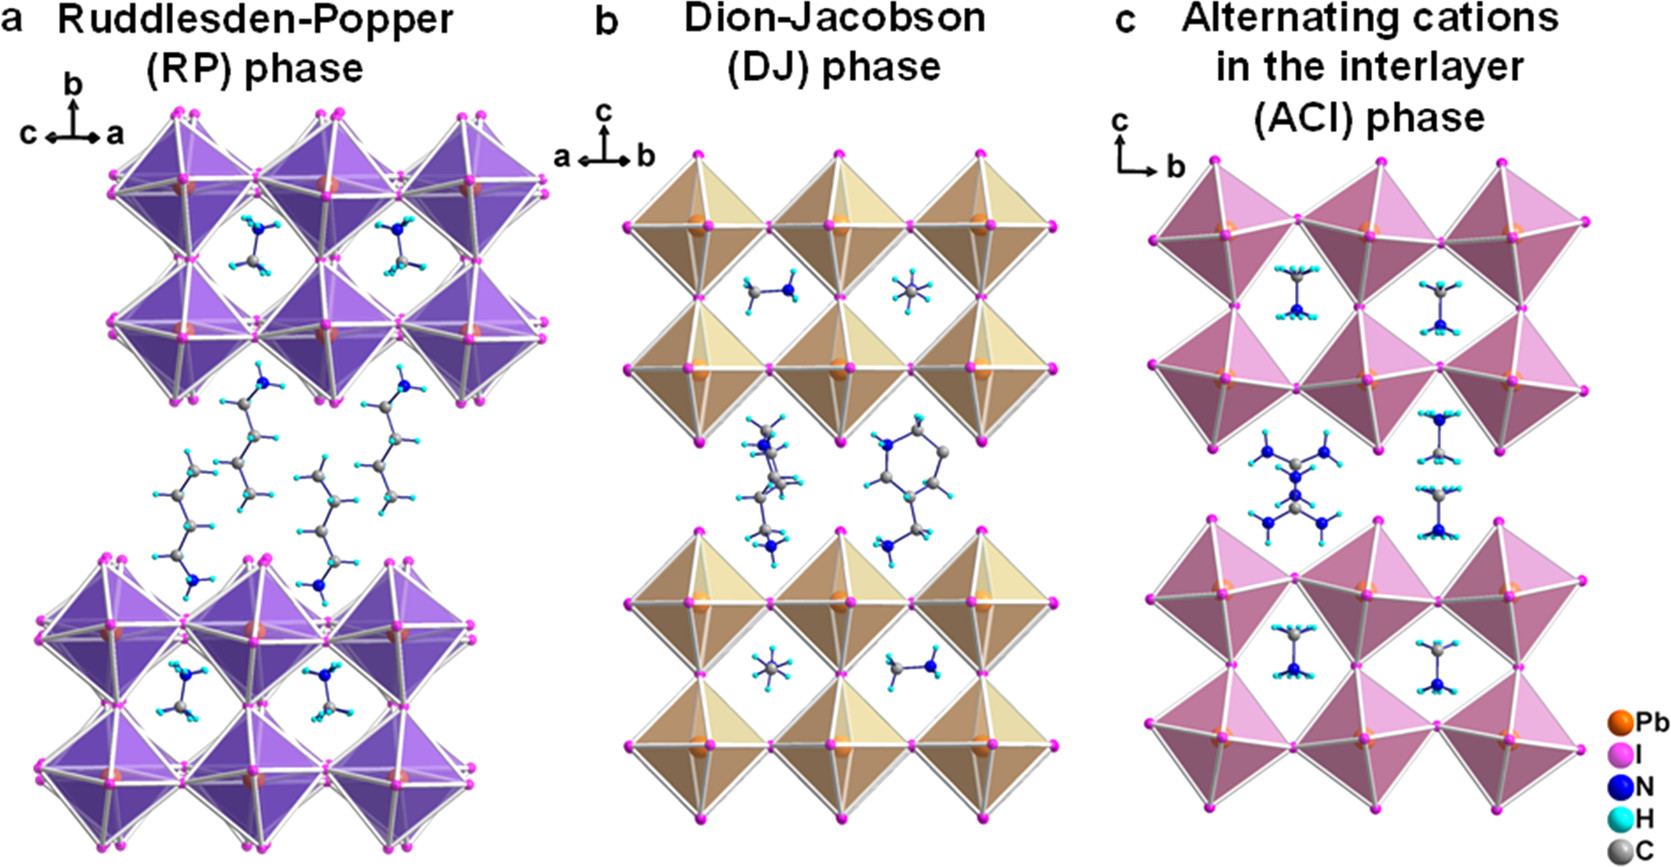
\includegraphics[width=0.9\textwidth]{figures/literature-review/figure2-10.png}
    \caption{Schematic illustration of different structural phases of 2D perovskites\cite{RN144}.}
    \label{fig:figure2.10}
\end{figure}

The \textbf{RP phase} represents the most extensively studied family of 2D perovskites and can be described by the general formula (A’)$_2$A$_{n-1}$M$_n$X$_{3n+1}$. Here, A′ is a bulky monovalent organic spacer cation, A is a smaller monovalent cation (as seen in 3D perovskites), M is a metal cation (e.g., Pb$^{2+}$, Sn$^{2+}$), and X is a halide anion. Two layers of organic spacers intercalate between the inorganic slabs, creating a van der Waals gap. While many RP-phase perovskites display an in-plane octahedral shift of (1/2, 1/2), more complex tilts and distortions can occur with bulky or flexible organic spacers. Despite potential drawbacks—such as restricted out-of-plane transport due to the van der Waals gap—RP perovskites are valued for their strong excitonic effects, tunable bandgaps, and suitability for light-emitting and photodetection applications\cite{RN108,RN190}.

The \textbf{DJ phase}, described by the formula A’A$_{n-1}$M$_n$X$_{3n+1}$, where A’ is typically a divalent organic spacer cation (e.g., diammonium compounds) with two ammonium tethering groups anchor to the inorganic layers. In contrast to the RP phase, DJ perovskites have only a single organic spacer layer between inorganic slabs, thus eliminating the van der Waals gap and often reducing the interlayer distance\cite{RN106}. This configuration improves out-of-plane electronic coupling and charge transport while strengthening hydrogen-bonding interactions—leading to excellent structural stability. Such attributes render DJ perovskites promising candidates for high-efficiency solar cells and transistors\cite{RN198}. 

The \textbf{ACI phase} is a relatively new structural motif where two different organic cations alternate between the inorganic layers, with the first example demonstrated in 2017\cite{RN214}. Often, the organic spacer cations are relatively small (comparable to methylammonium), resulting in shorter interlayer distances and stronger interlayer coupling\cite{RN242}. This structural motif can yield a reduced bandgap and enhanced charge transport, and there have been demonstrations of improved solar-cell efficiencies over comparable RP and DJ phases\cite{RN212,RN208}. However, because of stricter size constraints on the organic cations, the chemical space for ACI-phase perovskites is comparatively smaller.


\begin{figure}[ht]
    \centering
    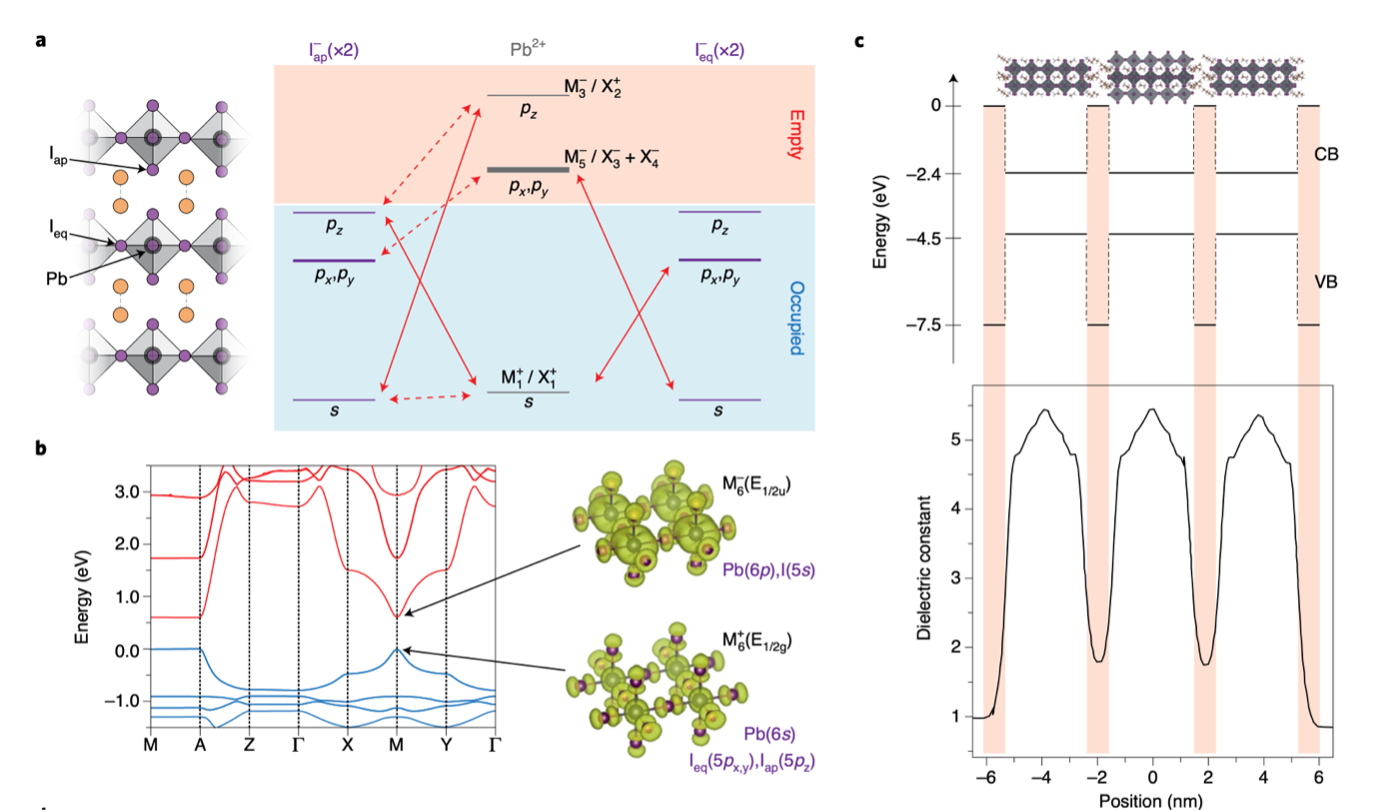
\includegraphics[width=\textwidth]{figures/literature-review/figure2-11.png}
    \caption{Electronic properties of 2D perovskites\cite{RN119}.}
    \label{fig:figure2.11}
\end{figure}

\textbf{Electronic Fundamentals}

The electronic structure of 2D perovskites is now relatively well understood, with their band edges predominantly governed by the inorganic layers and their structural and dielectric environment modulated by the organic spacers (Figure \ref{fig:figure2.11}). 

Generally, the bandgap widens as the thickness of the inorganic layer decreases (i.e., as n decreases). For example, monolayer (n = 1) perovskites typically exhibit bandgaps $\sim2.4$ eV, while quasi-2D structures with larger n values approach the bandgap of the corresponding 3D perovskite ($\sim1.5$ eV for MAPbI$_3$)\cite{RN199}. This tunability has been leveraged in studies to induce an “energy funneling” effect, where charge carriers move from wider-bandgap (lower-n) to narrower-bandgap (higher-n) regions, enhancing the efficiency of light-emitting diodes\cite{RN180}. Beyond structural thickness, the bandgap can also be finely tuned by altering the metal cation (M = Pb$^{2+}$, Sn$^{2+}$) or halide anion (X = I$^-$, Br$^-$, Cl$^-$)\cite{RN104}.



A defining feature that distinguishes 2D from 3D perovskites lies in the strong quantum confinement effects inherent to their layered structure\cite{RN385}. In 2D perovskites, the inorganic slabs act as quantum wells, while the organic layers serve as wide-bandgap barriers\cite{RN394}. This configuration leads to notably large exciton binding energies, ranging from 100 to 500 meV—substantially higher than the 10–50 meV typical of 3D perovskites—thus endowing 2D systems with pronounced excitonic behaviour advantageous for optoelectronic applications. However, the layered structure also induces highly anisotropic charge transport. In-plane transport benefits from robust orbital overlap between the metal and halide, often rivalling that in 3D perovskites (particularly for larger n values), whereas out-of-plane transport is hindered by the insulating organic layers acting as barriers to carrier motion\cite{RN119}.

\begin{figure}[ht]
    \centering
    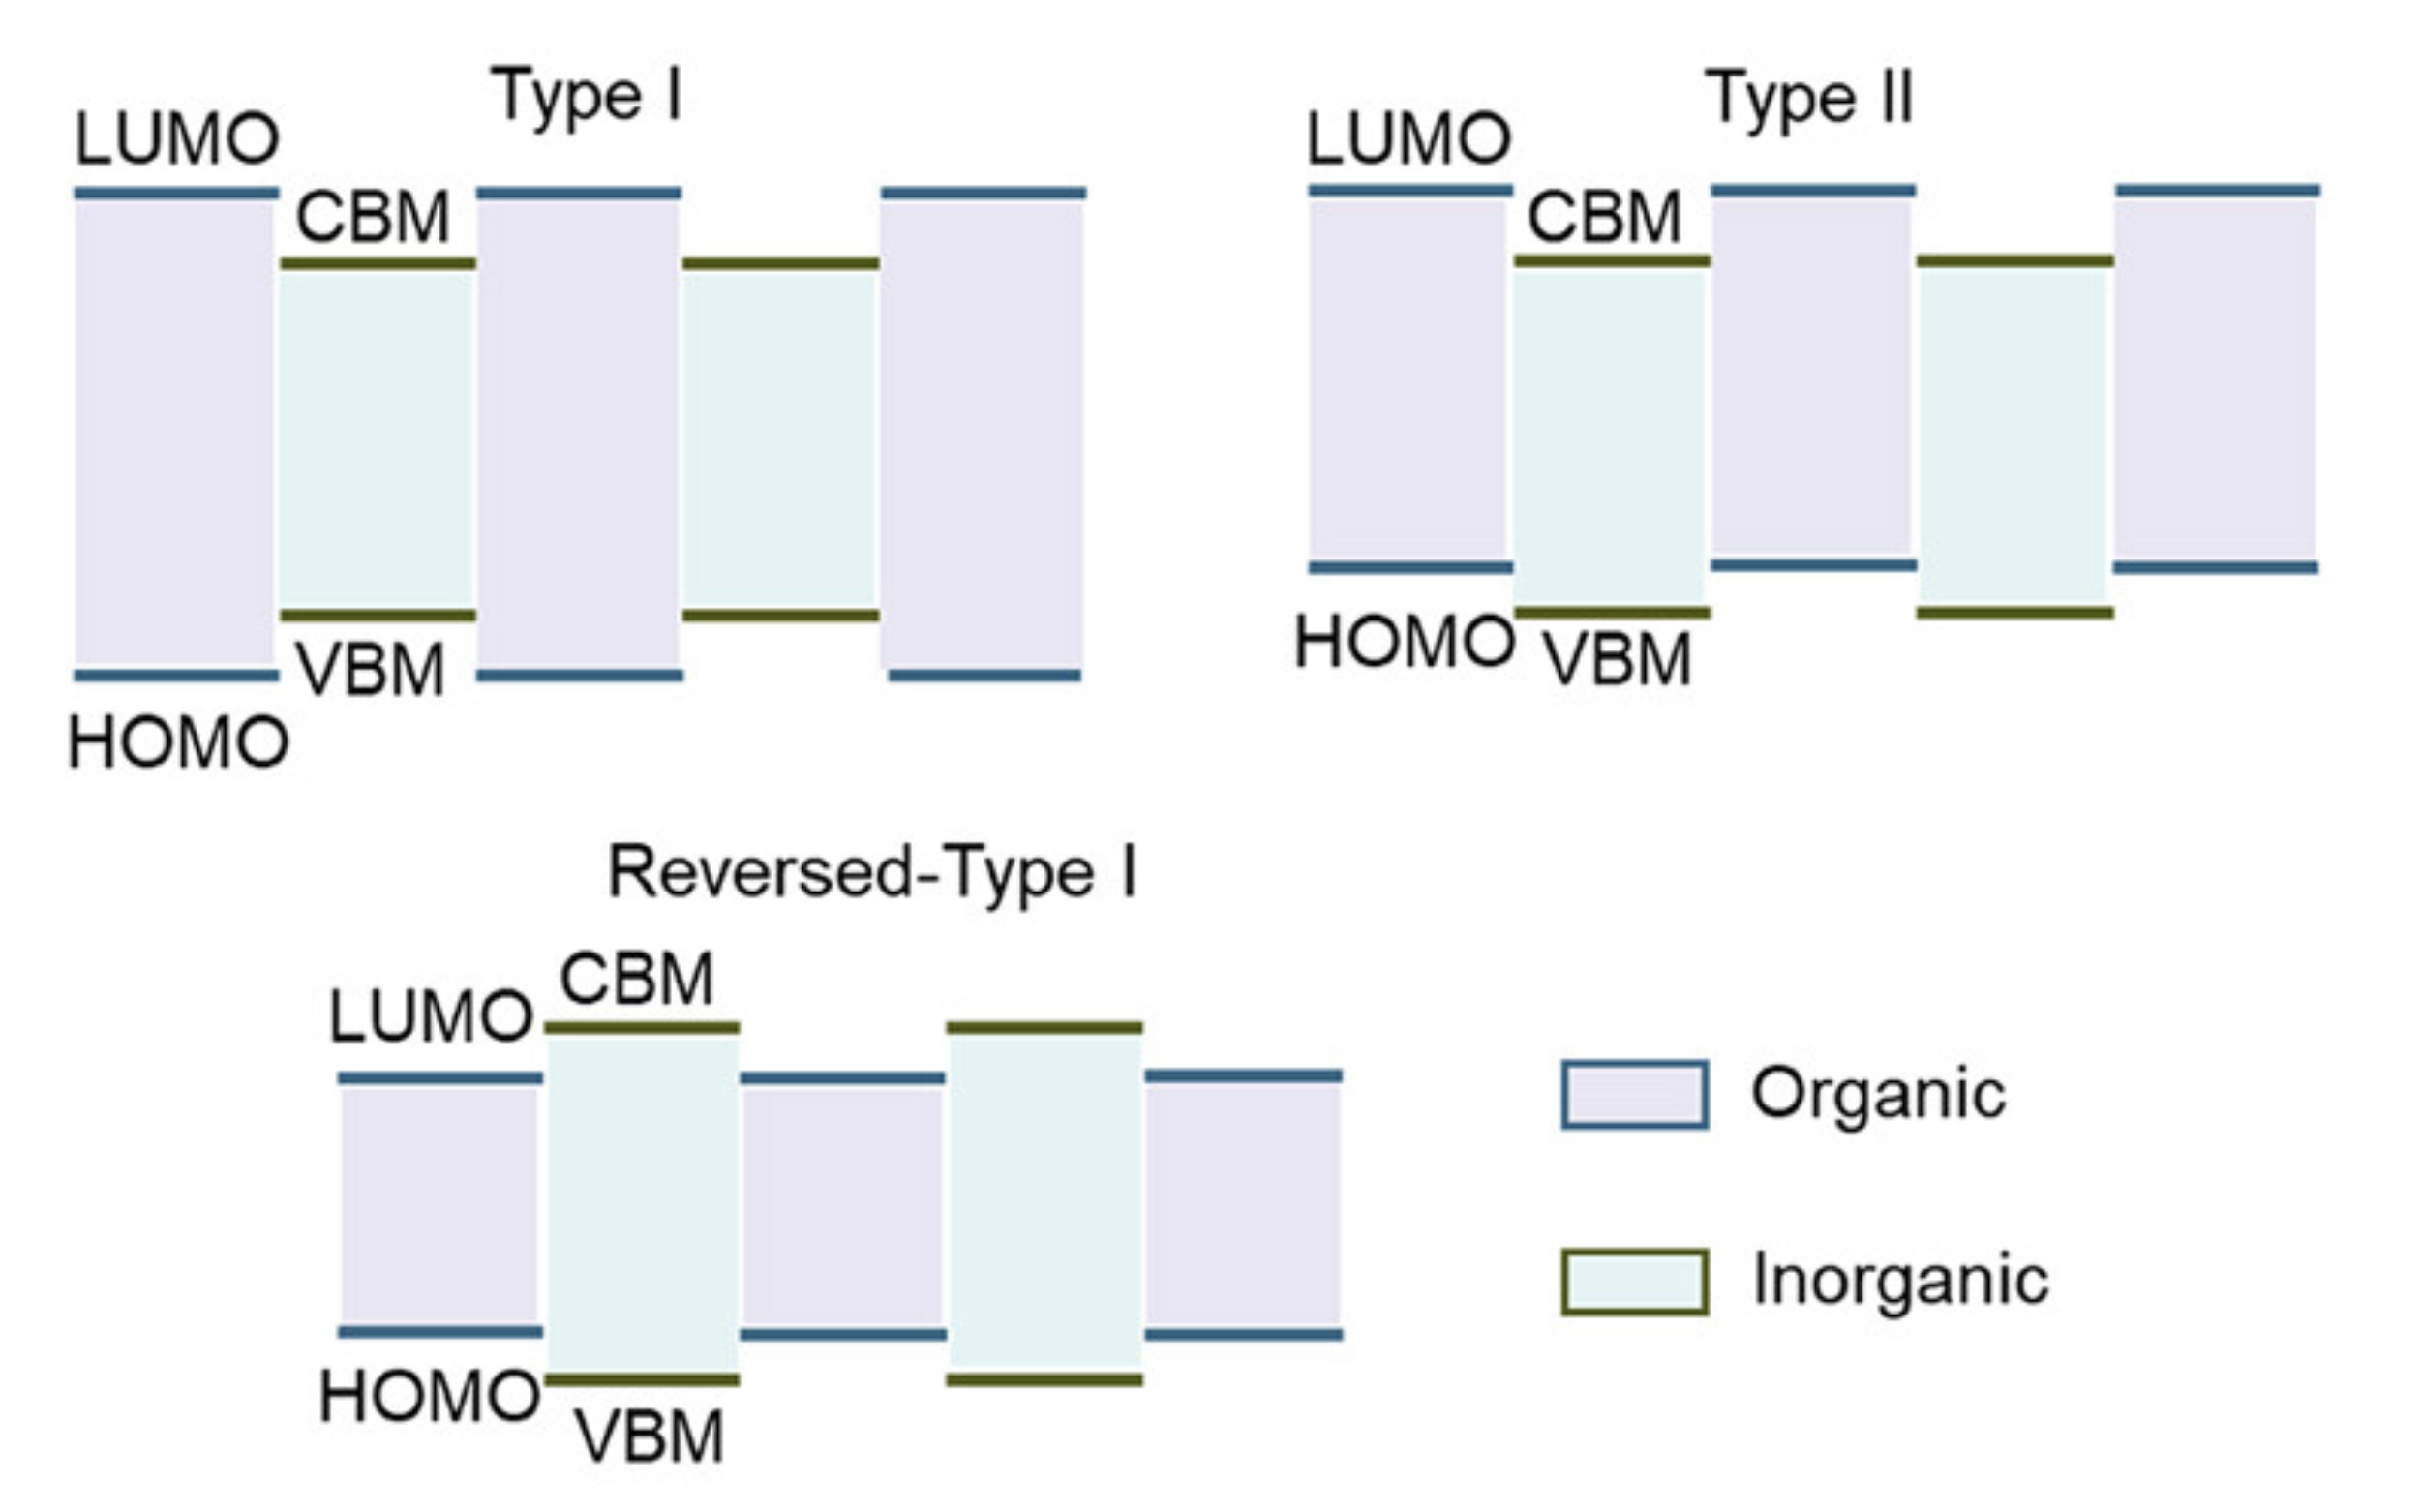
\includegraphics[width=0.9\textwidth]{figures/literature-review/figure2-12.png}
    \caption{Schematics of the quantum well effect in 2D perovskites\cite{RN304}.}
    \label{fig:figure2.12}
\end{figure}

One of the most actively explored strategies for improving 2D perovskite performance is tuning their quantum well structure through composition engineering. Energy-level alignments in these systems are generally categorized as type-I (straddling gap) or type-II (staggered gap), with four possible configurations. Most 2D perovskites naturally adopting a type-I configuration with organic component acts as the insulating barrier (Figure \ref{fig:figure2.12}). Research has explored various approaches to modulating energy level alignment, including altering the thickness and composition of the inorganic layer and tailoring the organic spacer design\cite{RN20,RN626,RN305}. Among these strategies, organic spacer engineering has emerged as the most promising, demonstrating the ability to achieve all four possible types of energy level alignment.

Despite these advancements, the tuning of energy level alignment remains limited, and many organic spacers have yet to be explored for further optimization. In the following section, we introduce design strategies for organic spacers to enhance their impact on perovskite properties.

\subsection{Design Strategies for Organic Spacers}

As mentioned above, the organic spacer cations in 2D perovskites play a pivotal role in determining their structural, electronic, and environmental stability properties. Rational design of these spacers enables the tuning of perovskite properties to optimize performance in optoelectronic devices.

The early discovery of organic spacers for 2D perovskites was largely serendipitous, driven by the limited availability of organic cations known to incorporate into the perovskite framework. Initial studies primarily focused on simple alkylammonium spacers, such as butylammonium (BA) and propylammonium (PA), with research efforts centred on varying spacer length or functional groups to improve film morphology and device performance\cite{RN135,RN504,RN217}. 

In recent years, spacer engineering has evolved significantly, shifting towards the deliberate design of organic cations with tailored functionalities. This includes the exploration of conjugated organic spacers, typically featuring aromatic systems such as benzene or thiophene rings\cite{RN218,RN31}. The introduction of conjugation has been shown to enhanced interactions between organic spacers, improved charge transport, and enable tunable optoelectronic properties\cite{RN228}. Additionally, spacer modification strategies now encompass functional group engineering—such as side-chain substitutions, fluorination, and positional adjustments of ammonium tethering groups—to finely control interlayer interactions, defect passivation, and environmental stability.

\begin{figure}[ht]
    \centering
    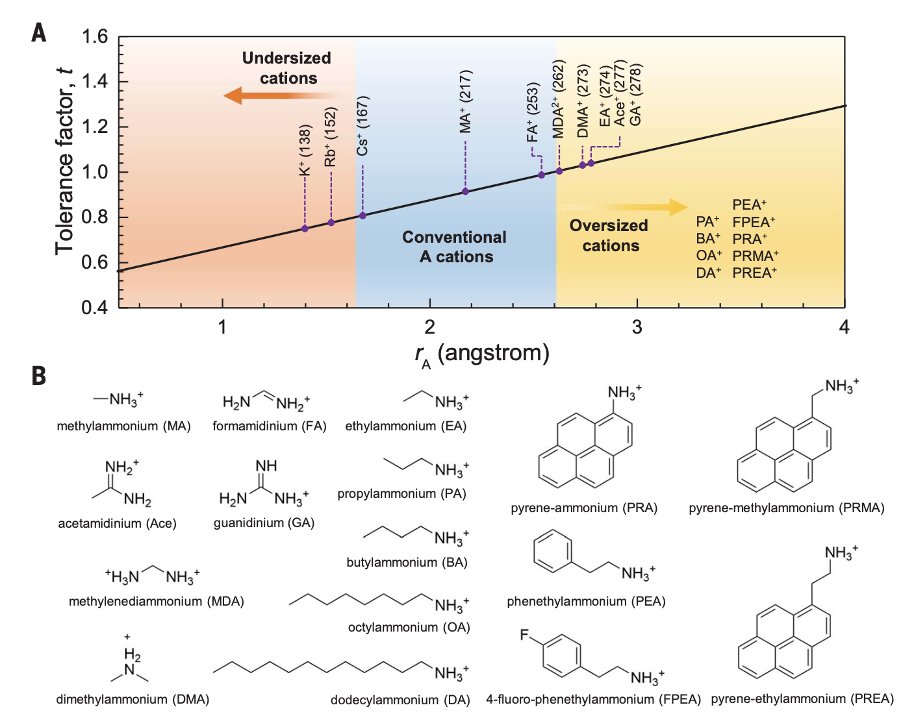
\includegraphics[width=\textwidth]{figures/literature-review/figure2-13.png}
    \caption{Molecular size constraints for organic spacers in 2D perovskites\cite{RN42}.}
    \label{fig:figure2.13}
\end{figure}

To maintain the perovskite framework, organic spacers must satisfy certain structural and chemical criteria. From a steric perspective, the size and shape of the organic spacer play a crucial role in determining whether it can fit within the inorganic framework and stabilize the 2D perovskite structure (Figure \ref{fig:figure2.13}). While there is no strict limitation on the length of the organic spacer—studies have successfully incorporated linear alkyl organic spacers with up to 18 carbon atoms into 2D perovskite framework\cite{RN637,RN638,RN639}—the cross-section area must remain within a certain threshold to avoid exceeding the available space within the 2D perovskite lattice\cite{RN519}. In particular, the cross-section width of the organic spacer, often approximated by the diameter of its conjugated backbone, should be smaller than width of the MX$_6$ octahedral unit\cite{RN20}. If the spacer is too bulky, studies have shown that it can lead to different structural dimensions or even disrupt the formation of a stable 2D lattice, leading to 0D or 1D perovskite\cite{RN640,RN641}.

Another critical consideration in designing organic spacers is the shape and configuration of the ammonium head group, which strongly influences hydrogen bonding. In 2D perovskites, this ammonium head typically fits into the cavity formed by the inorganic octahedral network, creating hydrogen bonds that stabilize the overall structure\cite{RN519,RN117}. The halide ions in the inorganic framework serve as hydrogen-bond acceptors, necessitating that the organic spacer contains a suitable hydrogen bond donor—typically an electron-deficient nitrogen bearing at least one hydrogen. Primary ammonium groups (i.e., $NH_3^+$) are widely used because they offer relatively strong hydrogen bonding, though secondary ($NH_2^+$) or tertiary ammonium group ($NH^+$) can also participate in hydrogen bond, albeit with generally lower bonding strength. Excessive steric hindrance around the nitrogen can impede its insertion into the inorganic pocket and weaken these critical bonds, potentially destabilizing the 2D perovskite. Typically, the hydrogen bond distance must remain below $\sim3.0-3.5 \AA$ to provide sufficient structural stabilization\cite{RN117}.

\begin{figure}[ht]
    \centering
    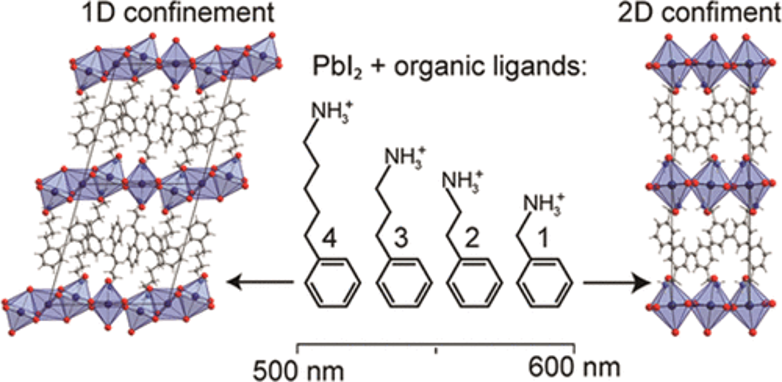
\includegraphics[width=0.9\textwidth]{figures/literature-review/figure2-14.png}
    \caption{Modulation of 2D perovskites formability by tuning linker length\cite{RN649}.}
    \label{fig:figure2.14}
\end{figure}

Recent work has demonstrated various strategies for modulating hydrogen bonding. In one study, researchers investigated organic spacers in which the ammonium tethering group was placed at different positions along the molecule, altering the distance between the ammonium head and the inorganic framework\cite{RN28}. The spacer with the weakest hydrogen bonding formed a one-dimensional (1D) perovskite, whereas the two stronger-bonding spacers yielded 2D structures. Another approach involved varying the length of linker segment between the ammonium head and the main body of the spacer, thereby increasing conformational flexibility and enhancing hydrogen-bond interactions with the inorganic lattice (Figure \ref{fig:figure2.14})\cite{RN86,RN649}. Additionally, functional group engineering—such as fluorination—has been shown to further strengthen hydrogen bonds, likely due to the high electronegativity and induced dipole moment of fluorine atoms\cite{RN211}.


Beyond the structural considerations necessary for forming a 2D perovskite, organic spacer engineering also provides opportunities to tailor electronic properties. In many cases, the organic spacer does not directly participate in the electronic structure of the inorganic framework, allowing it to act primarily as a structural template. For instance, shorter organic spacers can reduce the interlayer distance and thereby enhance out-of-plane charge transport\cite{RN179}. Additionally, adjustments to the inorganic octahedral tilting can further modulate the perovskite bandgap\cite{RN31}. Some conjugated organic cations—particularly those containing aromatic rings—are known to reduce energy barriers for charge transport relative to their alkyl-based counterparts\cite{RN239,RN88}.

\begin{figure}[ht]
    \centering
    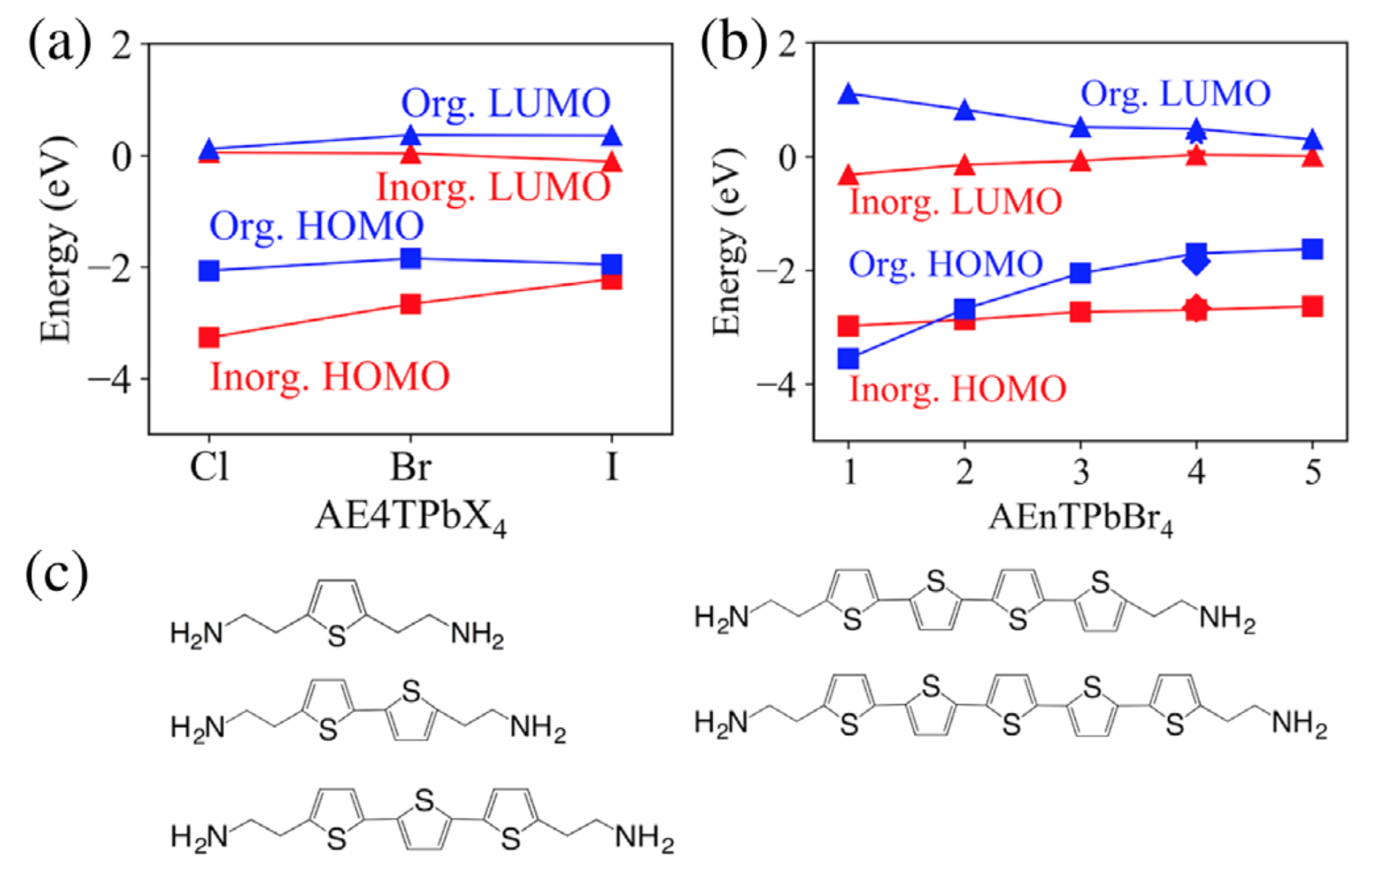
\includegraphics[width=\textwidth]{figures/literature-review/figure2-15.png}
    \caption{Engineering the energy level alignment in 2D perovskites by designing organic spacers\cite{RN18}.}
    \label{fig:figure2.15}
\end{figure}

Modifying the quantum well structure offers another route for electronic tuning. Introducing organic spacers with extended conjugation can shift the spacer’s frontier orbitals, potentially inverting the quantum-well alignment from type I to type II. Achieving this often requires complex spacer architectures with extended $\pi$-conjugation and functional-group modifications. In one study, organic cations featuring a $\pi$-conjugated pyrene backbone with varying linker lengths were introduced onto the perovskite surface. These cations contributed electronically to the surface band edges and influenced carrier dynamics, ultimately improving solar cell efficiency\cite{RN39}. In another series of studies (Figure \ref{fig:figure2.15}), oligothiophene-based organic spacers were incorporated into DJ-phase perovskites, with both DFT calculations and experimental results confirming that increasing the number of aromatic rings effectively tuned the energy-level alignment, leading to the realization of type-II alignment\cite{RN38,RN18}. Additionally, research on RP-phase perovskites has explored highly conjugated organic spacers, demonstrating that modifications to functional groups can achieve all four types of energy-level alignment. For instance, the introduction of electron-withdrawing units enabled type-II alignment, where the organic LUMO and inorganic VBM define the band edges. Meanwhile, incorporating a small bandgap unit facilitated a reversed type-I alignment\cite{RN20}. 

Despite the established design strategies for organic spacers in 2D perovskites, the optimization process remains highly complex. The intricate structural features of organic spacers, along with their interactions with the inorganic framework, introduce a vast number of variables that are challenging to fully understand through conventional trial-and-error methods or human intuition alone. To address this complexity, AI-driven approaches have emerged as powerful tools for accelerating material discovery and optimization. The following section explores recent advancements in AI-driven methodologies for 2D perovskites, with a particular emphasis on organic spacer design.

\subsection{AI-Driven Approaches for 2D perovskites}

ML methods have been extensively applied to the design of 3D perovskites, yet their use in guiding the discovery and optimization of 2D perovskites remains in a comparatively early stage. In 3D perovskites, a key focus has traditionally been an optimizing the inorganic frameworks—often represented by elemental compositions that are relatively straightforward for computational methods to handle\cite{RN314,RN422,RN317}. By contrast, 2D perovskites incorporate both inorganic layers and organic spacers. The design challenge therefore shifts prominently to selecting and engineering the organic spacer, which must meet specific geometric (e.g., size constraints) and chemical (e.g., functional group compatibility) requirements.

Given that ML-assisted discovery of 2D perovskites is still in its early stages, relevant studies in this field remain scarce. Therefore, to provide a broader perspective, below we review ML application in three closely related research areas: organic spacer design in 2D perovskites, hybrid materials interface design, and organic materials design. 

\begin{figure}[ht]
    \centering
    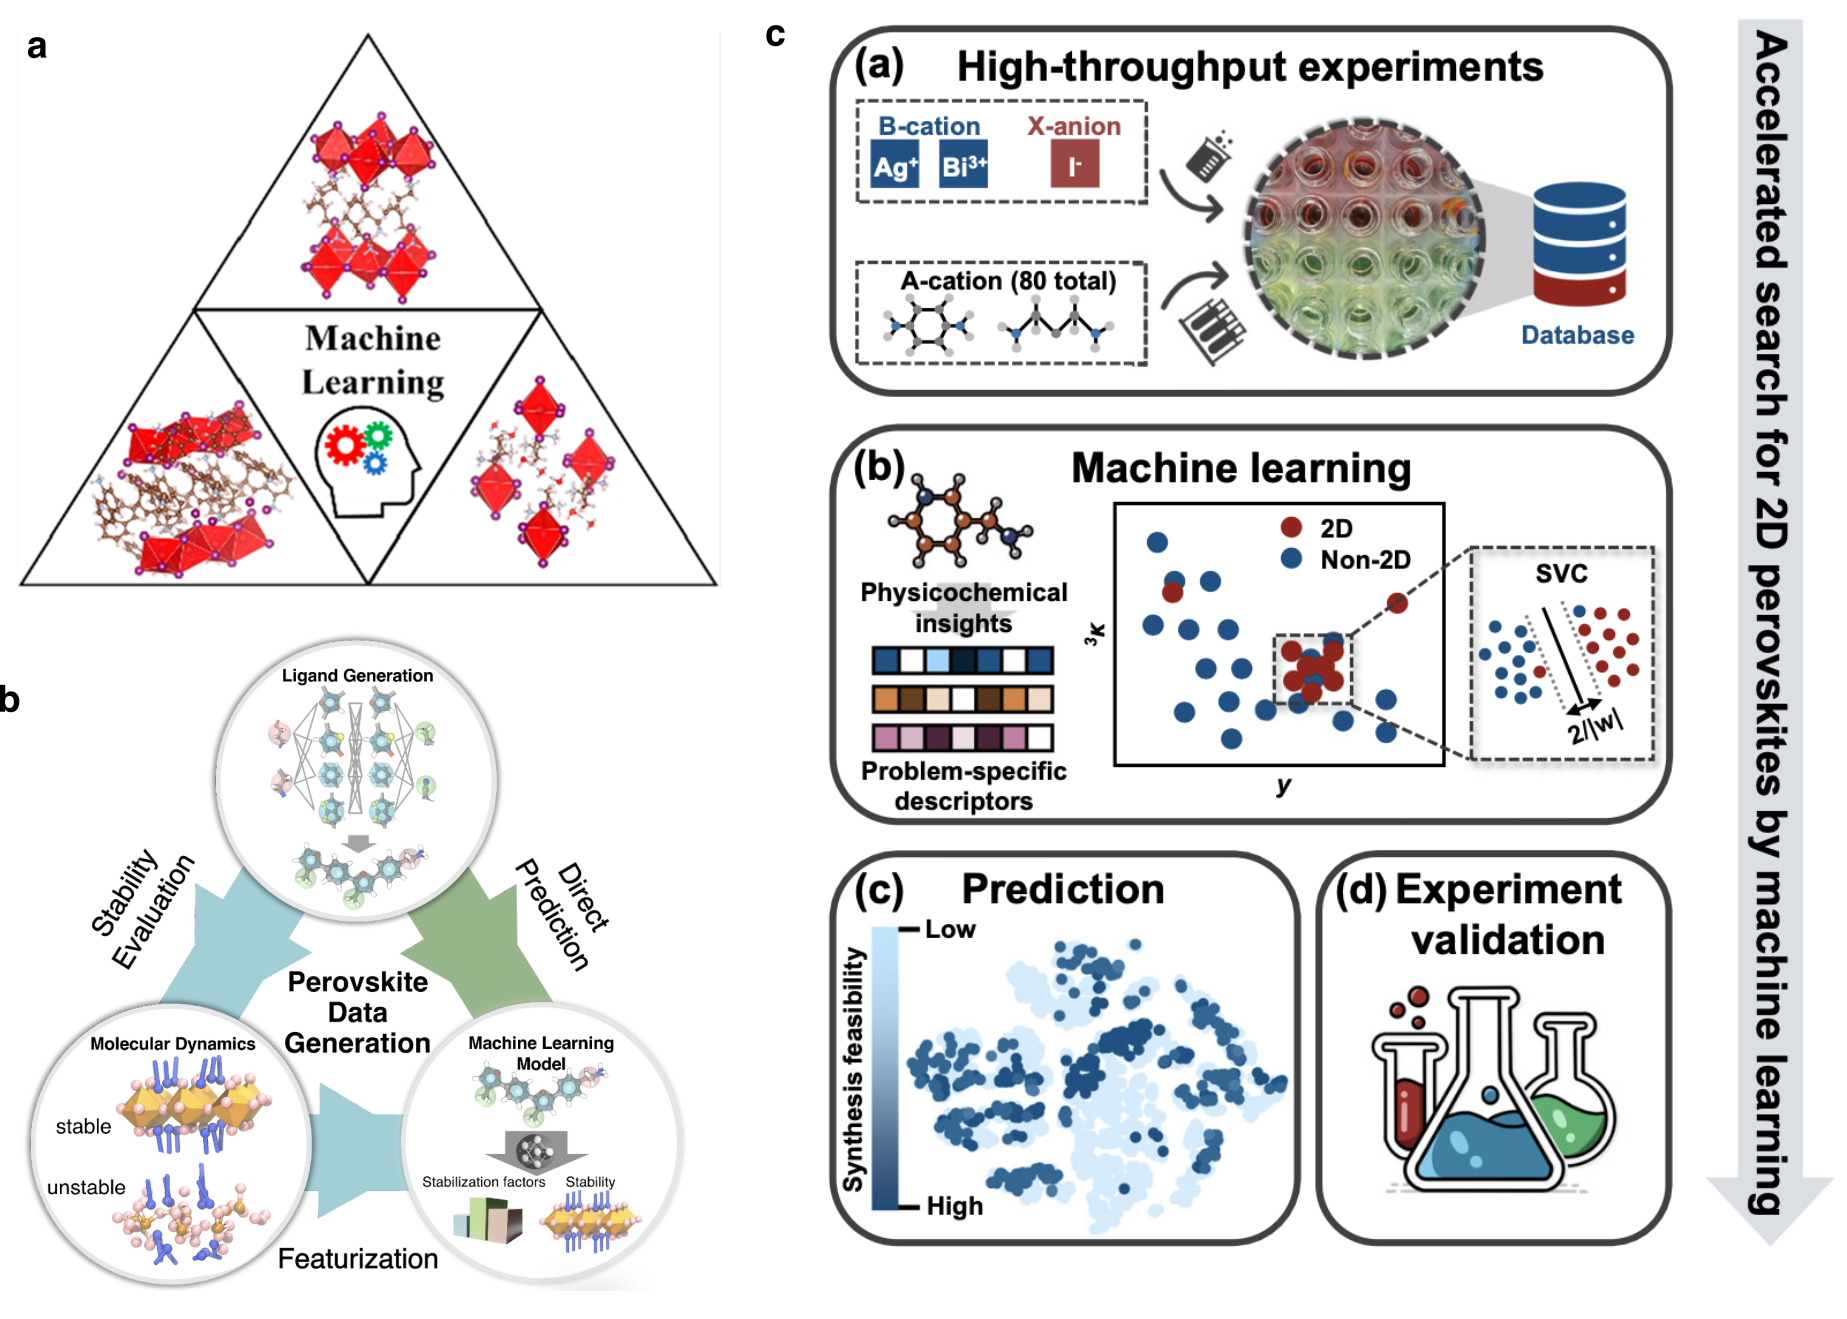
\includegraphics[width=\textwidth]{figures/literature-review/figure2-16.png}
    \caption{Machine learning workflows for 2D perovskite design\cite{RN283,RN12, RN315}.}
    \label{fig:figure2.16}
\end{figure}

The virtually unbounded chemical space of possible organic spacers has driven researchers to explore ML and other data-driven strategies for 2D perovskites (Figure \ref{fig:figure2.16}). An early study has used ML models trained on 86 reported organic spacers in lead-based 2D perovskites to derive design rules for predicting the perovskite dimensionality of five new organic spacers\cite{RN12}. Recent approaches have expanded the scope of spacer exploration considerably. For instance, Wu et al. utilized a ML model trained on 80 high throughput synthesized lead-free double perovskites to evaluate the synthesis feasibility of 8,460 organic spacers from PubChem\cite{RN315}. In another study, molecular dynamics simulations on over ten-thousand hypothetical organic spacers were used as training data to select six new ligands for perovskite synthesis\cite{RN283}. 


Beyond 2D perovskites, similar ML workflows have been applied to other hybrid materials interfaces involving small molecules, particularly in passivation materials for perovskite solar cells\cite{RN13,RN538,RN630}. In these studies, ML workflows typically follow a three-step approach. First, the physiochemical descriptors are selected based on domain knowledge. Second, the descriptors are computed from the organic molecule structure. Finally, these descriptors are used as input features for supervised machine learning models to predict key properties. For example, a recent study used various regression models to predict the power conversion efficiency (PCE) of perovskite solar cells passivated by ammonium salts, using a set of physiochemical descriptors\cite{RN538}. 

Compared to hybrid perovskites, ML-assisted design of organic materials is a relatively mature field, with well-established methods for molecular representation and advanced machine learning models\cite{RN612,RN563,RN610,RN564}. The most critical aspect of ML workflows in organic materials is how molecules are represented. Common molecular representations include: 

(1) SMILES (Simplified Molecular Input Line Entry System) – An invertible molecular representation widely used in text-based ML models. 

(2) Molecular fingerprints – Such as Morgan fingerprints or Extended Connectivity Fingerprints (ECFPs), which have been extensively applied to polymer design, peptide engineering, and organic emitter discovery. 

For instance, a recent study used a 2048-bit Morgan fingerprint to represent heat-resistant polymers, combined with a feed-forward neural network to down-select promising candidates from a virtual library\cite{RN610}. These representation techniques, combined with advanced ML models, have proven effective for guiding molecular design. However, directly applying these techniques to 2D perovskites is not straightforward due to the added complexity of the organic–inorganic interface.

A major limitation of the current ML approaches in 2D perovskites is their reliance on forward design workflows, which require exhaustive brute-force screening of chemical space. Since organic spacers must be predefined before descriptors can be calculated, the approach is not invertible, preventing direct generation of new molecular structures from target properties. Moreover, descriptor-based representations often fail to fully capture the molecular complexity of organic spacers. Such brute-force screening can be computationally expensive and may miss promising regions of chemical space if the initial library is not sufficiently diverse. Therefore, inverse design—where desired properties are defined a priori, and algorithms propose candidate molecules or structures—holds the promise of accelerating materials discovery for 2D perovskites. 

Furthermore, much of the pioneering ML work on 2D perovskites has been centred on questions of formability and stability, a critical gap remains in the application of AI-assisted workflow to predict physical properties of 2D perovskites. Energy level alignment, a key property controlling the spatial distribution and transfer of charge carriers and excitations in semiconducting materials and their interfaces, directly impacts the performance of optoelectronic devices. Different from well-studied elemental and compound semiconductors, organic and inorganic components in hybrid perovskites are heterogeneous with separate energetics, forming quantum-well-like structures\cite{RN18}. Although 2D perovskites have been investigated using traditional workflows, such as the Edisonian approach\cite{RN20} and high-throughput calculations\cite{RN236,RN617}, systematic exploration of the energy level alignment through AI-assisted approaches is still in its early stages\cite{RN618}, presenting a significant opportunity for advancement. 

\section{Summary and Research Gaps}\label{section:section2-3}

In the preceding sections, we introduced the two main pillars of this thesis: AI-assisted materials discovery—with particular attention to inverse design methodologies—and the design challenges posed by 2D perovskites, especially in the context of organic spacers. Their intersection is the central focus of this work.

From the perspective of 2D perovskite design, the vast chemical space of organic spacers necessitates the use of data-driven and machine learning techniques. These materials exhibit highly intricate structure–property relationships, with many potentially relevant features that are difficult to fully grasp through traditional approaches. To tackle this complexity, we focus on DJ-phase n=1 Pb–I-based perovskites as a prototype system for studying structure–property relationships. Insights gained from this prototype can then be generalized to other 2D perovskite phases and alternative inorganic frameworks. We choose energy level alignment as our target property, as it is crucial for optoelectronic applications yet remains insufficiently understood.

From the viewpoint of AI-assisted inverse materials design, this 2D perovskite system presents an equally compelling challenge. Unlike more extensively studied materials with large, well-curated datasets, 2D perovskites are relatively data-scarce and uniquely hybrid in nature, requiring careful consideration of both organic and inorganic components. While inverse design methodologies have shown promise for inorganic materials, organic molecules, and polymers, 2D perovskites introduce additional constraints—such as spacer size limitations and the complex organic–inorganic interface—that necessitate novel AI-driven approaches.

Moreover, the insights gained from this research could extend beyond 2D perovskites to a broader class of hybrid materials, where the intricate interplay between organic and inorganic components defines material properties. As emerging materials fields often suffer from data scarcity, developing machine learning strategies tailored to these challenges is essential. By leveraging AI in such contexts, we aim to contribute to a generalizable framework for hybrid material discovery, enabling data-driven innovation in materials science.

This thesis addresses several critical research gaps in the field of AI-driven 2D perovskite design:

\begin{itemize}
    \item Lack of large, high-quality datasets for 2D perovskites – Unlike well-established materials, 2D perovskites suffer from data scarcity. Existing datasets are often small, inconsistent, or lack standardization, limiting the ability of machine learning models to generalize effectively.
    \item Limited understanding of structure–property relationships – A quantitative and predictive understanding of how organic spacer chemistry influences electronic properties and synthesizability remains underdeveloped. The complexity of organic–inorganic interactions make it challenging to establish clear design rules.
    \item Challenges in inverse design for 2D perovskites – Existing inverse design models do not fully accommodate the unique constraints of hybrid materials, such as the size limitations of organic spacers and the chemical constraints associated with functional group compatibility.
    \item Challenges in AI-assisted approaches for hybrid materials – The absence of a standardized ML workflow for hybrid materials poses a significant barrier. Feature selection remains underdeveloped, and machine learning models struggle to encode key chemical and structural descriptors necessary for accurately modelling organic–inorganic interactions.
\end{itemize}

Addressing these challenges requires robust, AI-driven frameworks tailored to 2D perovskite design—particularly those that incorporate domain expertise, and feature property-driven design. The present thesis aims to bridge some of these gaps by exploring inverse design workflows that couple molecular design with inorganic framework constraints, ultimately accelerating the discovery of high-performance 2D perovskite materials.
